\documentclass{article}
\usepackage[letterpaper, top=1in, bottom=1in, left=1in, right=1in]{geometry}
\usepackage[utf8]{inputenc}

\usepackage[english]{babel}
\usepackage{tikz-cd, extarrows, esvect, esint, pgfplots, lipsum, bm, dcolumn}
\pgfplotsset{compat=1.18}
\usetikzlibrary{arrows}
\usepackage{amsmath, amssymb, amsthm, mathrsfs, mathtools, centernot, hyperref, fancyhdr, lastpage, mathabx}

\setlength{\parindent}{0pt} % set no indent
\hfuzz=5.002pt % ignore overfull hbox badness warnings below this limit

\renewcommand{\thispagestyle}[1]{}

\newtheorem{theorem}{Theorem}[section]
\newtheorem{proposition}[theorem]{Proposition}
\newtheorem{lemma}[theorem]{Lemma}
\theoremstyle{definition}
\newtheorem{example}{Example}[section]
\newtheorem{corollary}{Corollary}[theorem]
\theoremstyle{remark}
\newtheorem*{remark}{Remark}
\theoremstyle{definition}
\newtheorem{definition}{Definition}[section]
\renewcommand{\qed}{\hfill$\blacksquare$}
\renewcommand{\footrulewidth}{0.4pt}% default is 0pt


\begin{document}
\pagestyle{fancy}

\lhead{SLAM}
\chead{Muchang Bahng}
\rhead{\date{Spring 2023}}
\cfoot{\thepage / \pageref{LastPage}}

\title{Monocular Visual-Inertial Simultaneous Localization and Mapping (SLAM)}
\author{Muchang Bahng}
\date{Spring 2023}

\maketitle
\section{Introduction}

In computer vision, machines should reliably be able to see what the surrounding environment is like (\textbf{map building}) and where it is located in this environment (\textbf{localization}). Autonomous robots should know this in order to move around and do things. Vehicles should know this in order to reliably drive around. Mobile devices should implement this in order to produce stable holograms in augmented reality software. The general set of algorithms that allow machines to achieve this is called \textbf{Simultaneous Localization and Mapping (SLAM)}. 

In order to solve this mapping and localization situation, we can implement \textbf{intrusive sensors} in a prepared environment, which are effective but very limited (e.g. QR codes, guiding rails). On the other hand, \textbf{non-intrusive sensors} allow for robots to explore more general environments, but are more difficult to implement. We will focus on non-intrusive sensors since we cannot presume which environment our machine will be in (though we generally know whether it is indoors or outdoors). 

Therefore, a typical visual SLAM workflow includes the following steps: 
\begin{enumerate}
    \item \textbf{Sensor data acquisition}: Acquisition and preprocessing of camera images (along with IMU sensors, etc.) 
    \item \textbf{Visual Odometry (VO)}: Estimating the camera movement between adjacent frames to estimate the displacement of the observer (\textbf{ego-motion}) and generate a rough local map. Known as \textbf{frontend}. This tends to be noisy and accumulates error. 
    \item \textbf{Backend Filtering/Optimization}: The backened receievs camera poses and different time stamps from VO and results from loop closing, and then applies optimization to generate a fully optimized trajectory and map. Known as \textbf{backend}. 
    \item \textbf{Loop Closing}: Determines whether the robot has returned to its previous position in order to reduce accumulated drift. If a loop is detected, it will provide information to backend for further optimization. 
    \item \textbf{Reconstruction}: Constructs the map based on camera trajectory. 
\end{enumerate}
Ideally, we would want SLAM to process images at 30fps, which is generally considered real-time. 

\subsection{Hardware}

\subsubsection{Sensors}

There are many types of sensors we should be familiar with: 
\begin{enumerate}
    \item \textbf{GPS} uses satellites and triangulation to locate a specific point on the Earth's surface. But this is not good for indoors. 
    \item \textbf{LIDAR} shoots beams of light and measures the return time, like echolocation but with light. They are usually bulky and slightly expensive, used mainly in vehicles. 
    \item \textbf{Cameras} take pictures/videos for visual data. There are many types of cameras: 
    \begin{enumerate}
        \item \textbf{Monocular cameras} uses only one camera. It is cheap but it is hard to measure depth from the projection of $\mathbb{R}^3$ to $\mathbb{R}^2$. If we want to recover the 3D structure, we have to change the camera's view angle, but it only does it on a relative scale. 
        \item \textbf{Stereo cameras} use two cameras, and the distance between these two is called the \textbf{baseline}. The depth is calculated from the disparity of the two image pairs. 
        \item \textbf{RGB-D (RGB-Depth) Cameras} measures the distance between objects and the camera by actively emitting light to the object and receiving it back. 
        \item \textbf{Opti-track cameras} (usually multiple ones) are placed around a certain area and can use software to detect feature points on a rigid body or skeleton. 
\end{enumerate}
    \item \textbf{IMU (Inertial Measurement Unit)} consists of a \textbf{gyroscope}, which measures the orientation and angular velocity, and an \textbf{accelerometer}, which measures the acceleration. This is known as a 6 DoF IMU, but if we have a \textbf{magnetometer}, which measures magnetic fields, this is known as a 9 DoF IMU. IMUs are actually quite cheap and are incorporated into many commercial mobile devices, but they tend to be very noisy, so their data is usually optimized with feature detection algorithms. 
\end{enumerate}
The machine could receive lots of different data, e.g. inertial data, photos, LIDAR, but we will mainly focus on camera data (continuous stream of pictures) coupled with other sensors. The goal of visual SLAM is to localize and build a map using this continuous stream of images. The type of lens also matter since they can cause distortion effects. 
\begin{enumerate}
    \item \textbf{Pinhole lens} is just a pin hole in which the light passes through. 
    \item \textbf{Fisheye lens} are ultra wide-angle lens that produces strong visual distortion intended to create a wide panoramic or hemispherical image.
\end{enumerate}
Either way, we model our data as a projection of the real world onto some light sensor that goes through the lens, followed by some random noise which we assume to be Gaussian. 

\subsubsection{Wireless Connections}

When looking at edge assisted SLAM, the strength and reliability of the connections between the mobile agent and the edge server is important. These are usually done over WiFi or cellular. 
\begin{enumerate}
    \item WiFi uses multiple bands of radio waves to provide high-speed internet access to mobile devices. It is necessary to have a modem connected to a router, and a device needs a wireless adapter to translate between data and radio signals. WiFi-5G provides faster speeds over shorter range, and WiFi-2.4G provides slower speeds over larger range. 
    \item Cellular uses cell phone towers to enable mobile device communication. Cellular 5G, 4G, and LTE are the top choices. 
\end{enumerate}

\subsubsection{Memory}

For fast retrieval, the data is stored in RAM rather than an SSD. The server would store a global map and other info in a 16GB to 256GB RAM. 
\subsection{Image Processing}
 
\subsubsection{Feature Extraction}

Analyzing an entire picture pixel-by-pixel can be too computationally intensive, which is why we can extract certain \textbf{feature points} that represent the image. In essence, we extract feature points from images and match them between consecutive images to estimate things like camera motion (for VO) and the scene structure (for mapping). 

Colloquially, feature points are like special points in an image, which tend to be corners, edges, or pixels that may be different from its neighbors. In 1988, corners were good feature points because we can observe a significant gradient change in all directions. On the other hand, a flat region has no gradient change and an edge region has no gradient changed along the edge direction. This paradigm manifested in the \textbf{Harris Corner Detector} algorithm. 

However, just detecting corners can be very naive, especially when camera angles have changed, so more sophisticated feature extraction algorithms, like SIFT, SURF, and ORB, have been introduced. Compared with simple corner points, these features should have certain properties: 
\begin{enumerate}
    \item \textbf{Repeatability}: the same feature could be found in different images. 
    \item \textbf{Distinctiveness}: different features have different expressions. 
    \item \textbf{Efficiency}: the number of feature points should be far fewer than the number of pixels. 
    \item \textbf{Locality}: the feature is only related to a small image area. 
\end{enumerate}
SIFT and SURF have been patented, are too computationally intensive, and are too slow, so they are not used for real-time SLAM. However, the more recently developed \textbf{ORB} (Oriented FAST and rotated BRIEF) algorithm is widely used due to its speed and open-sourceness, resulting in ORB-SLAM. 

The \textbf{FAST} algorithm takes a pixel $p$ and compares the brightness of $p$ to surrounding 16 pixels within a radius. They are divided into three classes (darker, lighter, or similar to $p$), and if more than $8$ pixels are darker or brighter than $p$ then it is selected as a keypoint. 
\begin{center}
    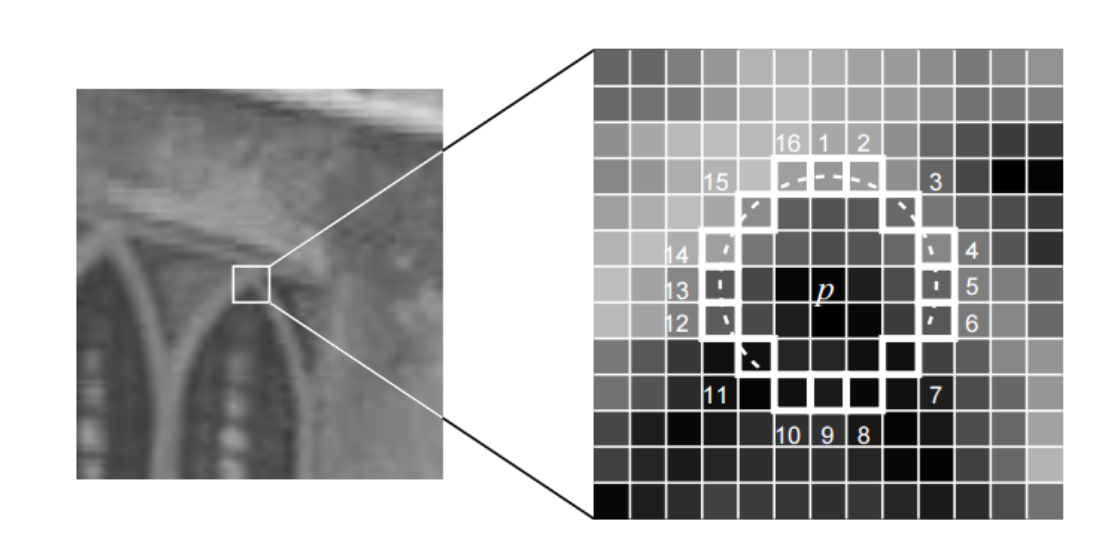
\includegraphics[scale=0.2]{img/FAST_points.png}
\end{center}
However, FAST features do not have an orientation component and multiscale features. So \textbf{ORB} algorithm uses a multiscale image pyramid. An image pyramid is a multiscale representation of a single image, that consist of sequences of images all of which are versions of the image at different resolutions. Each level in the pyramid contains the downsampled version of the image than the previous level. Once orb has created a pyramid it uses the fast algorithm to detect keypoints in the image. By detecting keypoints at each level orb is effectively locating key points at a different scale. In this way, ORB is partial scale invariant. 
\begin{center}
    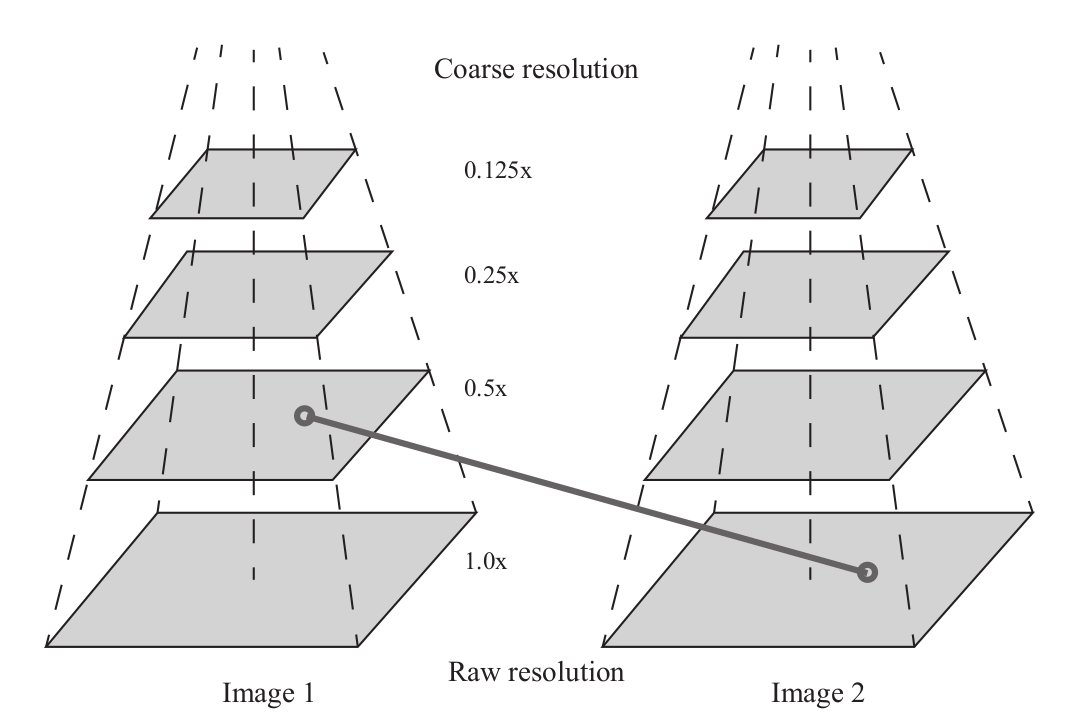
\includegraphics[scale=0.2]{img/image_pyramid.png}
\end{center}
After locating keypoints orb now assign an orientation to each keypoint like left or right facing depending on how the levels of intensity change around that keypoint. For detecting intensity change orb uses intensity centroid. The intensity centroid assumes that a corner’s intensity is offset from its center, and this vector may be used to impute an orientation. 

\subsubsection{Segmentation}

Another image processing algorithm uses convolutional neural networks to classify the pixels in an image to certain classes. 
\begin{enumerate}
    \item \textbf{Semantic segmentation} labels specific regions of an image according to a corresponding \textit{class} (e.g. fruit, person) of what is being represented. 
    \item \textbf{Instance segmentation} separates different \textit{instances} of an image for each instance. It goes beyond just semantic segmentation. 
\end{enumerate}
ORB-SLAM2 and ORB-SLAM3 (the latest ORB-SLAM algorithms) do not implement segmentation since they assume that we are working in a static environment (i.e. with no moving parts like walking humans). Map building with features that are actively moving in the environment would be very problematic, so algorithms like edgeSLAM segments frames between moving and static parts, and runs visual odometry on those feature points within the static portions. Something to keep in mind is incorrectly labeling a static part as moving isn't too problematic, but if we incorrectly label a moving part as static and attempt to construct a map from it, we would get very bad results. 

Another application of segmentation is that we can train these neural nets further on camera data to increase classification accuracy within the environment, minimizing the false positives and especially the false negatives. 

\subsubsection{Types of Maps}

There are two types of maps. \textbf{Topological maps} are simply graphs composed of nodes and edges. It relaxes the requirements on precise locations on a map by removing map details and emphasizes whether the nodes are connected or not. It is more compact but not good for representing complex maps. \textbf{Metric maps} emphasizes the exact numerical locations of the objects in maps. They may be represented as a \textbf{point cloud} composed of a bunch of map points in $\mathbb{R}^3$, and the number of points in which we consider determine how sparse or dense they are. 
\begin{enumerate}
    \item \textbf{Sparse maps} do not use many points and do not express all the objects. They focus on modeling certain classes of objects, which gives quick representations. They are mainly used in SLAM algorithms due to their speed and because we can still retrieve useful local information from these maps. 
    \begin{center}
        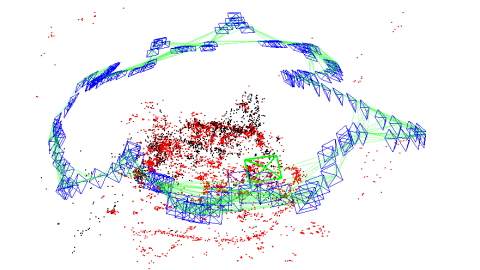
\includegraphics[scale=0.5]{img/sparse_map.png}
    \end{center}
    
    \item \textbf{Dense maps} focus on modeling \textit{all} the things that are seen in a frame and has much more map points than a sparse map. They are quite slow to make, but for accurate navigation this is what we need. 
    \begin{center}
        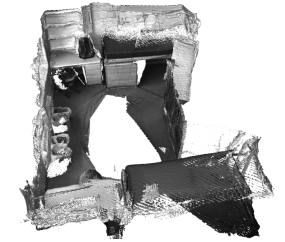
\includegraphics[scale=0.5]{img/dense_map.png}
    \end{center}
\end{enumerate}

\section{Transformations}

It is well known that a rigid body transformation has 6 degrees of freedom (3 orientation + 3 translation). Our goal is to write a compact representation of this group of transformations. 

\subsection{Special Orthogonal and Euclidean Groups}
Note that given some point $\mathbf{p} \in \mathbb{R}^3$, we can have multiple representations of it based on the coordinate system we're using. We are really interested in two orthonormal bases: 
\begin{enumerate}
    \item The \textbf{world coordinate system}, which is just some stationary inertial coordinate marked with the subscript $W$. 
    \[\mathbf{p_W} = x_W \mathbf{e_x^W} + y_W \mathbf{e_y^W} + z_W \mathbf{e_z^W} \] 
    
    \item The \textbf{camera coordinate system}, which is a \textit{moving} coordinate system. The $z$-axis of the camera coordinate system is usually perpendicular to the camera lens. 
    \[\mathbf{p_C} = x_C \mathbf{e_x^C} + y_C \mathbf{e_y^C} + z_C \mathbf{e_z^C} \] 
\end{enumerate}
Note that we can go from the world and camera coordinate system by rotations and translations. Ignoring translations for now, we can get 
\[ \mathbf{p} = \begin{pmatrix} | & | & | \\ \mathbf{e_x^W} & \mathbf{e_y^W} & \mathbf{e_z^W} \\ | & | & | \end{pmatrix} \begin{pmatrix} x_W \\ y_W \\ z_W \end{pmatrix} = \begin{pmatrix} | & | & | \\ \mathbf{e_x^C} & \mathbf{e_y^C} & \mathbf{e_z^C} \\ | & | & | \end{pmatrix} \begin{pmatrix} x_C \\ y_C \\ z_C \end{pmatrix} \]
where the matrices are of $\mathbf{R} \in \mathrm{O}(3)$, which means $\mathbf{R}^T = \mathbf{R}^{-1}$, so we have the change of basis transformation: 
\[\begin{pmatrix} x_W \\ y_W \\ z_W \end{pmatrix} = \begin{pmatrix} (\mathbf{e_x^W})^T \mathbf{e_x^C} & (\mathbf{e_x^W})^T \mathbf{e_y^C} & (\mathbf{e_x^W})^T \mathbf{e_z^C} \\ 
(\mathbf{e_y^W})^T \mathbf{e_x^C} & (\mathbf{e_y^W})^T \mathbf{e_y^C} & (\mathbf{e_y^W})^T \mathbf{e_z^C} \\ 
(\mathbf{e_z^W})^T \mathbf{e_x^C} & (\mathbf{e_z^W})^T \mathbf{e_y^C} & (\mathbf{e_z^W})^T \mathbf{e_z^C}
\end{pmatrix} \begin{pmatrix} x_C \\ y_C \\ z_C \end{pmatrix} \]
Therefore, to go between $\mathbf{p_W}$ and $\mathbf{p_C}$, we just have to use some rotation matrix $\mathbf{R} \in \mathrm{SO}(3)$. However, there are translations $\mathbf{t}$, so we extend this to the special euclidean group $\mathrm{SE}(3)$, of form 
\[\mathrm{SE}(3) = \bigg\{ \mathbf{T} = \begin{pmatrix} \mathbf{R} & \mathbf{t} \\ \mathbf{0}^T & 1 \end{pmatrix} \in \mathbb{R}^{4 \times 4} \mid \mathbf{R} \in \mathrm{SO}(3), \; \mathbf{t} \in \mathbb{R}^3 \bigg\}\]
That is, given some vector $\mathbf{a}_1 \in \mathbb{R}^3$, the transformation $\mathbf{a}_2 = \mathbf{R} \mathbf{a}_1 + \mathbf{t}$ is equivalent to simply multiplying \
\[\begin{pmatrix} \mathbf{a}_2 \\ 1 \end{pmatrix} = \begin{pmatrix} \mathbf{R} & \mathbf{t} \\ \mathbf{0}^T & 1 \end{pmatrix} \begin{pmatrix} \mathbf{a}_1 \\ 1 \end{pmatrix} \]
This forms a group, with inverse formula given by 
\[\mathbf{T}^{-1} = \begin{pmatrix} \mathbf{R}^T & -\mathbf{R}^T \mathbf{t} \\ \mathbf{0}^T & 1 \end{pmatrix}\]
The transformation $\mathbf{T}_{21}$ is from system $1$ to $2$ (read right to left, like matrix multiplication). 

\subsection{Rotation Vectors and Euler Angles}
Another representation of a 3D rigid body rotation is with a 3D vector that is parallel with the axis of rotation and the length is equal to the angle of rotation. That is, we can get a vector of form $\theta \mathbf{n}$, where $\mathbf{n}$ is a unit vector and $\theta$ is the angle of rotation. There is a clear bijection (given that $\theta$ is defined on a quotient space) between rotation vectors and $\mathrm{SO}(3)$: 
\begin{enumerate}
    \item Vector to Matrix
    \[\mathbf{R} = \cos{\theta} \mathbf{I} + (1 - \cos{\theta}) \mathbf{n} \mathbf{n}^T + \sin{\theta} \begin{pmatrix} 0 & -n_3 & n_2 \\ n_3 & 0 & -n_1 \\ -n_2 & n_1 & 0 \end{pmatrix} \]
    \item Matrix to Vector: $\mathbf{n}$ is the normalized eigenvector of $\mathbf{R}$ of eigenvalue $1$, and 
    \[\theta = \mathrm{arccos}\bigg( \frac{\mathrm{tr}(\mathbf{R}) - 1}{2} \bigg)\]
\end{enumerate}

Euler angles express the rotation across each axis, and the order of rotation must be specified (since $\mathrm{SO}(3)$ is not abelian).  
\begin{enumerate}
    \item Rotate around $Z$ axis: $\theta_{\mathrm{yaw}} = y$ 
    \item Rotate around $Y$ axis: $\theta_{\mathrm{pitch}} = p$ 
    \item Rotate around $X$ axis: $\theta_{\mathrm{roll}} = r$
\end{enumerate}
Therefore, we can use the 3-dimensional vector $(y, p, r)^T$ to describe any rotation, but due to the \textit{Gimbal lock} problem, a degree of freedom is lost in singularity cases. So this is not a good method for simulation, and is only good for human-to-computer interaction. It turns out that no $3$-dimensional representation of $SO(3)$ exists that avoids this singularity problem. However, there is a $4$-dimensional one. 

\subsection{Quaternions}

The quaternions are numbers $\mathbf{q} = q_0 + q_1 i + q_2 j + q_3 k$ that satisfy 
\begin{align*}
    i^2 &= j^2 = k^2 = -1 \\
    ij &= k, ji = -k \\
    jk &= i, kj = -i \\
    ki &= j, ik = -j 
\end{align*}
More specifically, it is an associative normed ring. Let us define the operations. Given two quaternions 
\begin{align*}
    \mathbf{q}_a & = [s_a, \mathbf{v}_a]^T = s_a + x_a i + y_a j + z_a k \\
    \mathbf{q}_a & = [s_b, \mathbf{v}_b]^T = s_b + x_b i + y_b j + z_b k 
\end{align*}
\begin{enumerate}
    \item Addition is defined 
    \[\mathbf{q}_a + \mathbf{q}_b = [s_a + s_b, \mathbf{v}_a + \mathbf{v}_b]^T\]
    
    \item Scalar multiplication is defined 
    \[c \mathbf{q}= [k s, k\mathbf{v}]^T\]
    
    \item Multiplication is defined by distributing over all elements
    \begin{align*}
    \mathbf{q}_a \mathbf{q}_b & = s_a s_b - x_a x_b - y_a y_b - z_a z_b \\
    & + (s_a x_b + x_a s_b + y_a z_b - z_a y_b) i \\
    & + (s_a y_b - x_a z_b + y_a s_b + z_a x_b) j \\
    & + (s_a z_b + x_a y_b - y_a x_b + z_a s_b) k 
    \end{align*}
    
    \item The norm is defined 
    \[||\mathbf{q}_a || = \sqrt{s_a^2 + x_a^2 + y_a^2 + z_a^2}\]
    
    \item Conjugate is defined 
    \[\mathbf{q}_a^{*} = s_a - x_a i - y_a j - z_a k\]
    
    \item The inverse is the formula 
    \[\mathbf{q}^{-1} = \frac{\mathbf{q}^*}{||\mathbf{q}||^2}\]
\end{enumerate}
A rotation of a vector $\mathbf{p}$ is $\mathbf{R}\mathbf{p}$ where $\mathbf{R} \in \mathrm{SO}(3)$, and we can represent a rotation of $\mathbf{p}$ with a unit quaternion $\mathbf{q}$. We take the imaginary quaternion $[0, \mathbf{p}]^T$ and multiply it as such
\[\mathbf{p}^\prime = \mathbf{q} \mathbf{p} \mathbf{q}^{-1}\]
and take the imaginary part of $\mathbf{p}^\prime$. The conversion between $\mathbb{R}$ and $\mathbb{q}$ is quite involved, so we will not mention it here. 

\subsection{More General Transformations}

So note that the degrees of freedom for a rotation is $3$ (though it cannot be represented with $3$ parameters; $4$ must be provided at least in quaternion form). Along with the $3$ translation parameters, 
\begin{enumerate}
    \item the degrees of freedom of the Euclidean transformation group $\mathrm{SO}(3)$ is $6$. Length, angle, and volume are all invariant. 
    \[\mathrm{SE}(3) = \bigg\{ \mathbf{T} = \begin{pmatrix} \mathbf{R} & \mathbf{t} \\ \mathbf{0}^T & 1 \end{pmatrix} \in \mathbb{R}^{4 \times 4} \mid \mathbf{R} \in \mathrm{SO}(3), \; \mathbf{t} \in \mathbb{R}^3 \bigg\}\]
    
    \item the degrees of freedom of the similarity transformation group is $7$ ($+1$ for scaling). Volume ratio is invariant. 
    \[\bigg\{ \mathbf{T} = \begin{pmatrix} s \mathbf{R} & \mathbf{t} \\ \mathbf{0}^T & 1 \end{pmatrix} \in \mathbb{R}^{4 \times 4} \mid \mathbf{R} \in \mathrm{SO}(3), \; s \in \mathbb{R}, \; \mathbf{t} \in \mathbb{R}^3 \bigg\}\]
    
    \item the degrees of freedom for the affine transformation semigroup (not always invertible) is $12$ ($9$ for general linear mapping, plus $3$ for translation). Parallelism and volume ratio is invariant. 
    \[\bigg\{ \mathbf{T} = \begin{pmatrix} \mathbf{A} & \mathbf{t} \\ \mathbf{0}^T & 1 \end{pmatrix} \in \mathbb{R}^{4 \times 4} \mid \mathbf{A} \in \mathbb{R}^{3 \times 3}, \; \mathbf{t} \in \mathbb{R}^3 \bigg\}\]
    
    \item the degrees of freedom for the perspective transformations are $15$ ($+3$ for scale $\mathbf{a}$). Under this, plane intersection and tangency is invariant, and this is what is most similar to a camera lens. 
    \[\bigg\{ \mathbf{T} = \begin{pmatrix} \mathbf{A} & \mathbf{t} \\ \mathbf{a}^T & 1 \end{pmatrix} \in \mathbb{R}^{4 \times 4} \mid \mathbf{A} \in \mathbb{R}^{3 \times 3}, \; \mathbf{t} \in \mathbb{R}^3, \; \mathbf{a} \in \mathbb{R}^3 \bigg\}\]
\end{enumerate}

\subsection{Lie Groups}

Recall that the exponential of a matrix is defined 
\[\exp(\mathbf{A}) = \sum_{k=0}^\infty \frac{1}{k!} \mathbf{A}^k\]
and the inverse logarithm map acting on $\mathbf{R} \in \mathrm{SO}(3)$ is 
\[\ln(\mathbf{R}) = \sum_{k=0}^n \frac{(-1)^k}{k + 1} (\mathbf{R} - \mathbf{I})^{k+1}\]
$\mathrm{SO}(3)$ and $\mathrm{SE}(3)$ are all Lie groups, which are really smooth manifolds, and therefore we can look at their tangent space at the origin $\mathbf{0}$, which is by definition the Lie algebra. A Lie algebra $\mathfrak{g}$ of a Lie group $\mathcal{G}$ is a vector space equipped with a Lie bracket: an alternating bilinear map $[ \cdot, \cdot] : \mathfrak{g} \times \mathfrak{g} \longrightarrow \mathfrak{g}$ satisfying the Jacobi identity 
\[\forall \;  \mathbf{X}, \mathbf{Y}, \mathbf{Z} \; [\mathbf{X}, [\mathbf{Y}, \mathbf{Z}]] + [\mathbf{Z}, [\mathbf{X}, \mathbf{Y}]] + [\mathbf{Y}, [\mathbf{Z}, \mathbf{X}]] = \mathbf{0}\]
Usually, we will work with the algebra of matrices, which has matrix multiplication equipped, and define the Lie bracket to be the commutator 
\[[\mathbf{X}, \mathbf{Y}] = \mathbf{X} \mathbf{Y} - \mathbf{Y} \mathbf{X}\]
The set of all traceless $3 \times 3$ real matrices of the form
\[\boldsymbol{\phi} = \begin{pmatrix} 0 & - \phi_3 & \phi_2 \\ \phi_3 & 0 & -\phi_1 \\ - \phi_2 & \phi_1 & 0 \end{pmatrix}\]
forms the Lie algebra $\mathfrak{so}(3)$ of the Lie group $\mathrm{SO}(3)$. It is a $3$-dimensional vector space. Since $\mathfrak{so}(3)$ is isomorphic to $\mathbb{R}^3$, sometimes writers denote the elements as simply $3$-vectors rather than a full matrix. It turns out that the Lie algebra $\mathfrak{se}(3)$ of $\mathrm{SO}(3)$ is the $6$-dimensional vector space of matrices of form
\[\mathfrak{se}(3) = \bigg\{ \boldsymbol{\xi} = \begin{pmatrix} \boldsymbol{\phi} & \boldsymbol{\rho} \\ \mathbf{0}^T & 0 \end{pmatrix} \in \mathbb{R}^{4 \times 4} \; \bigg| \; \boldsymbol{\phi} \in \mathfrak{so}(3), \; \boldsymbol{\rho} \in \mathbb{R}^3 \bigg\}\]
which can be represented by a $6$-vector. Now the relationship between adding two vectors in the Lie algebras exponentiating them vs exponentiating them first and multiplying is given by the BCH formula 
\[\ln\big( \exp(\mathbf{A}) \exp(\mathbf{B}) \big) = \mathbf{A} + \mathbf{B} + \frac{1}{2} [ \mathbf{A}, \mathbf{B}] + \frac{1}{12} [ \mathbf{A}, [\mathbf{A}, \mathbf{B}]] - \frac{1}{12} [\mathbf{B}, [\mathbf{A}, \mathbf{B}]] + \ldots\]

\subsection{Camera Parameterization}

Now we can use this transformations to describe how the 3D world gets transformed into a matrix representing an image. There are 3 stages: 
\begin{enumerate}
    \item \textbf{World-to-Camera}: 3D-3D projection. Rotation, Scaling, Translation. 
    \item \textbf{Camera-to-Image}: 3D-2D projection. Loss of information. Depends on the camera model and parameters (pinhole, f-theta, etc.). 
    \item \textbf{Image-to-Pixel}: Continuous to Discrete. Quantization and origin shift. 
\end{enumerate}

Now, let us have some position vector in the world coordinate system $\mathbf{p}_W = (x_W, y_W, z_W)^T$, since the coordinates are usually the standard basis $\mathbf{e}_1, \mathbf{e}_2, \mathbf{e}_3$. Given that the camera is facing at some $\mathbf{R} \in \mathrm{SO}(3)$ and translated $\mathbf{t} \in \mathbb{R}^3$ units, $\mathbf{p}$ in the camera coordinate system is 
\[\mathbf{p}_C = \mathbf{R} \mathbf{p}_W + \mathbf{t}\]
or more compactly, we can write 
\[\begin{pmatrix} \mathbf{p}_C \\ 1 \end{pmatrix} = \begin{pmatrix} \mathbf{R} & \mathbf{t} \\ \mathbf{0}^T & 1 \end{pmatrix} \begin{pmatrix} \mathbf{p}_W \\ 1 \end{pmatrix}\]
where the $4 \times 4$ transformation matrix is known as the \textbf{camera extrinsic matrix}. This extrinsic matrix can change if the physical location/orientation of the camera is changed, making it a function of time $\mathbf{T}(t)$. 

The pinhole model projects the 3D points in the camera coordinate system into a 2D plane, shown as a yellow plane below. The rays pass the center of the camera opening and are projected on the 2D plane on the other end. The 2D plane is what is captured as images by the camera. It is a lossy transformation, which means projecting the points from the camera coordinate system to the 2D plane can not be reversed (the depth information is lost — Hence by looking at an image captured by a camera, we can’t tell the actual depth of the points). The X and Y coordinates of the points are projected onto the 2D plane. The 2D plane is at f (focal-length) distance away from the camera.  The projection Xi, Yi can be found by the law of similar triangles (the ray entering and leaving the camera center has the same angle with the x and y-axis, alpha and beta respectively), giving us 
\[\frac{x_i}{f} = \frac{x_C}{z_C} \text{ and } \frac{y_i}{f} = \frac{y_C}{z_C}\]
Technically, there should be a minus sign, but we can ignore it for all practical purposes. 
\begin{center}
    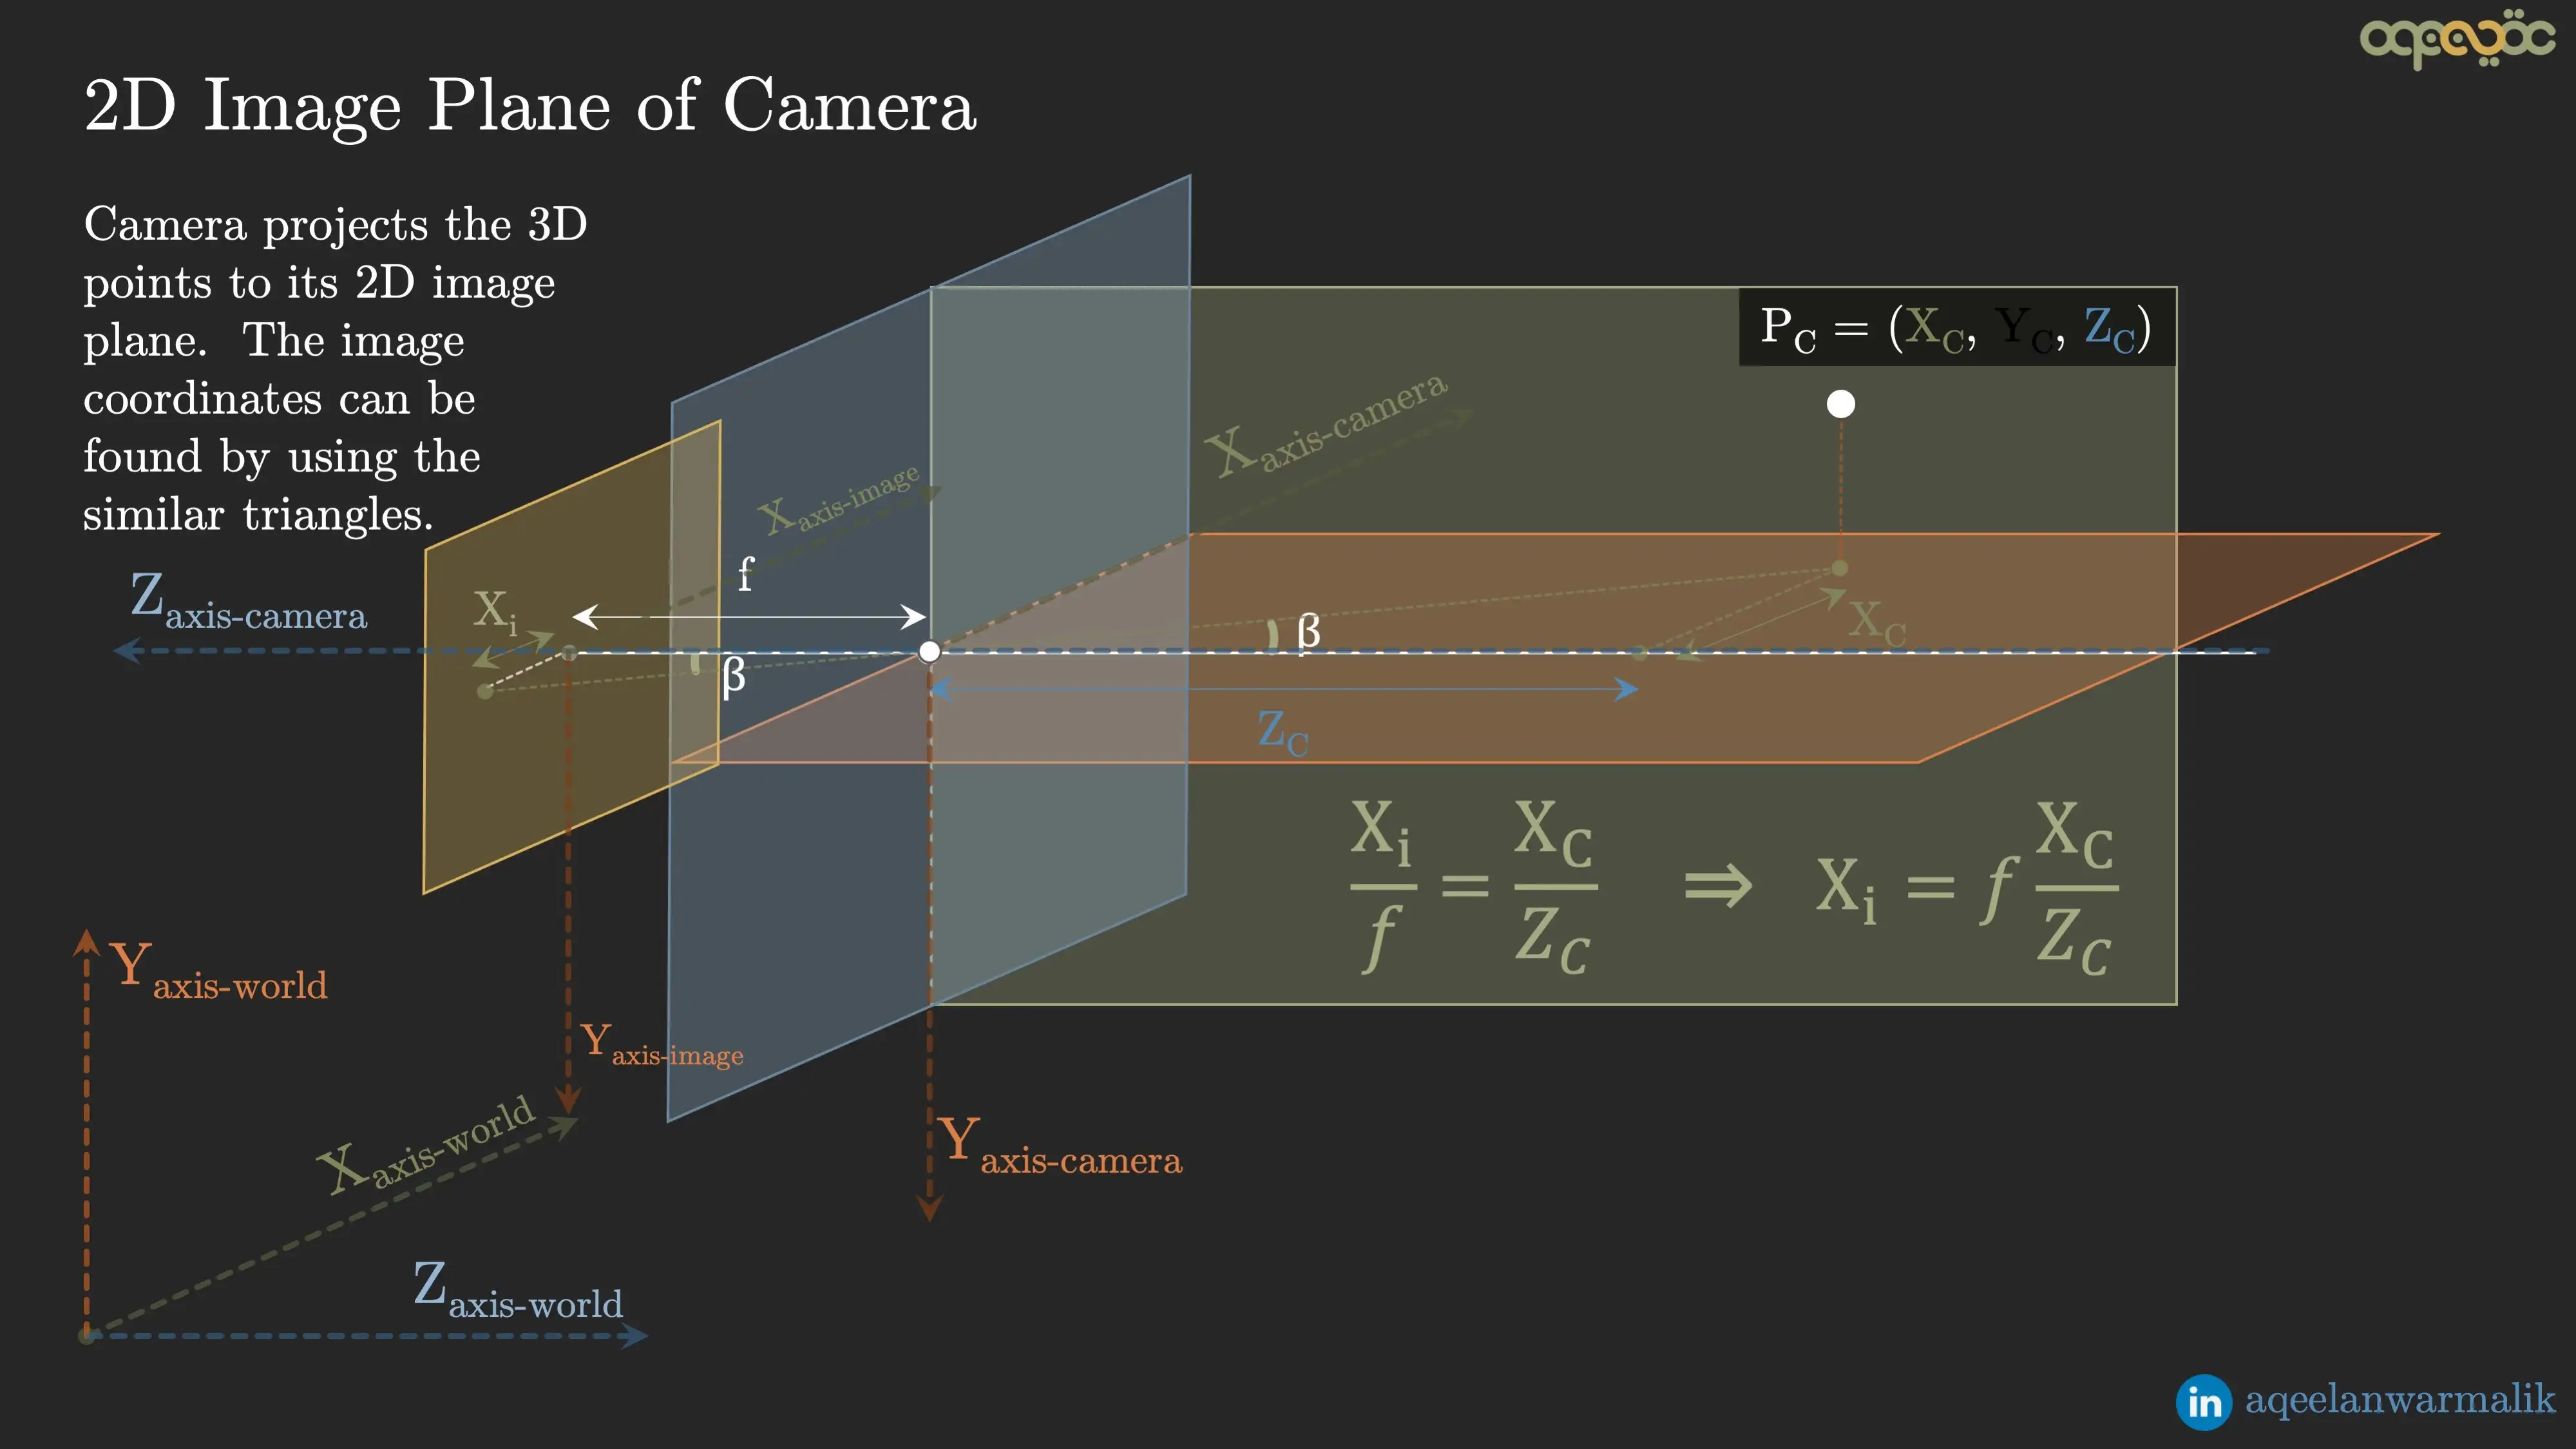
\includegraphics[scale=0.08]{img/X_triangle.png}
\end{center}
So if we know the actual 3D points in the camera coordinates ($x_C, y_C, z_C$ known) and the focal length $f$, then we can simply calculate the image plane to be 
\[x_i = f \frac{x_C}{z_C} \text{ and } y_i = f \frac{y_C}{z_C}\]
which can be modeled by the matrix equation in homogeneous coordinates
\[\begin{pmatrix} x_i \\ y_i \\ 1 \end{pmatrix} = \begin{pmatrix} f/z_C & 0 & 0 & 0 \\ 0 & f/z_C & 0 & 0 \\ 0 & 0 & 1/z_C & 0 \end{pmatrix} \begin{pmatrix} x_C \\ y_C \\ z_C \\ 1 \end{pmatrix} \]
\begin{center}
    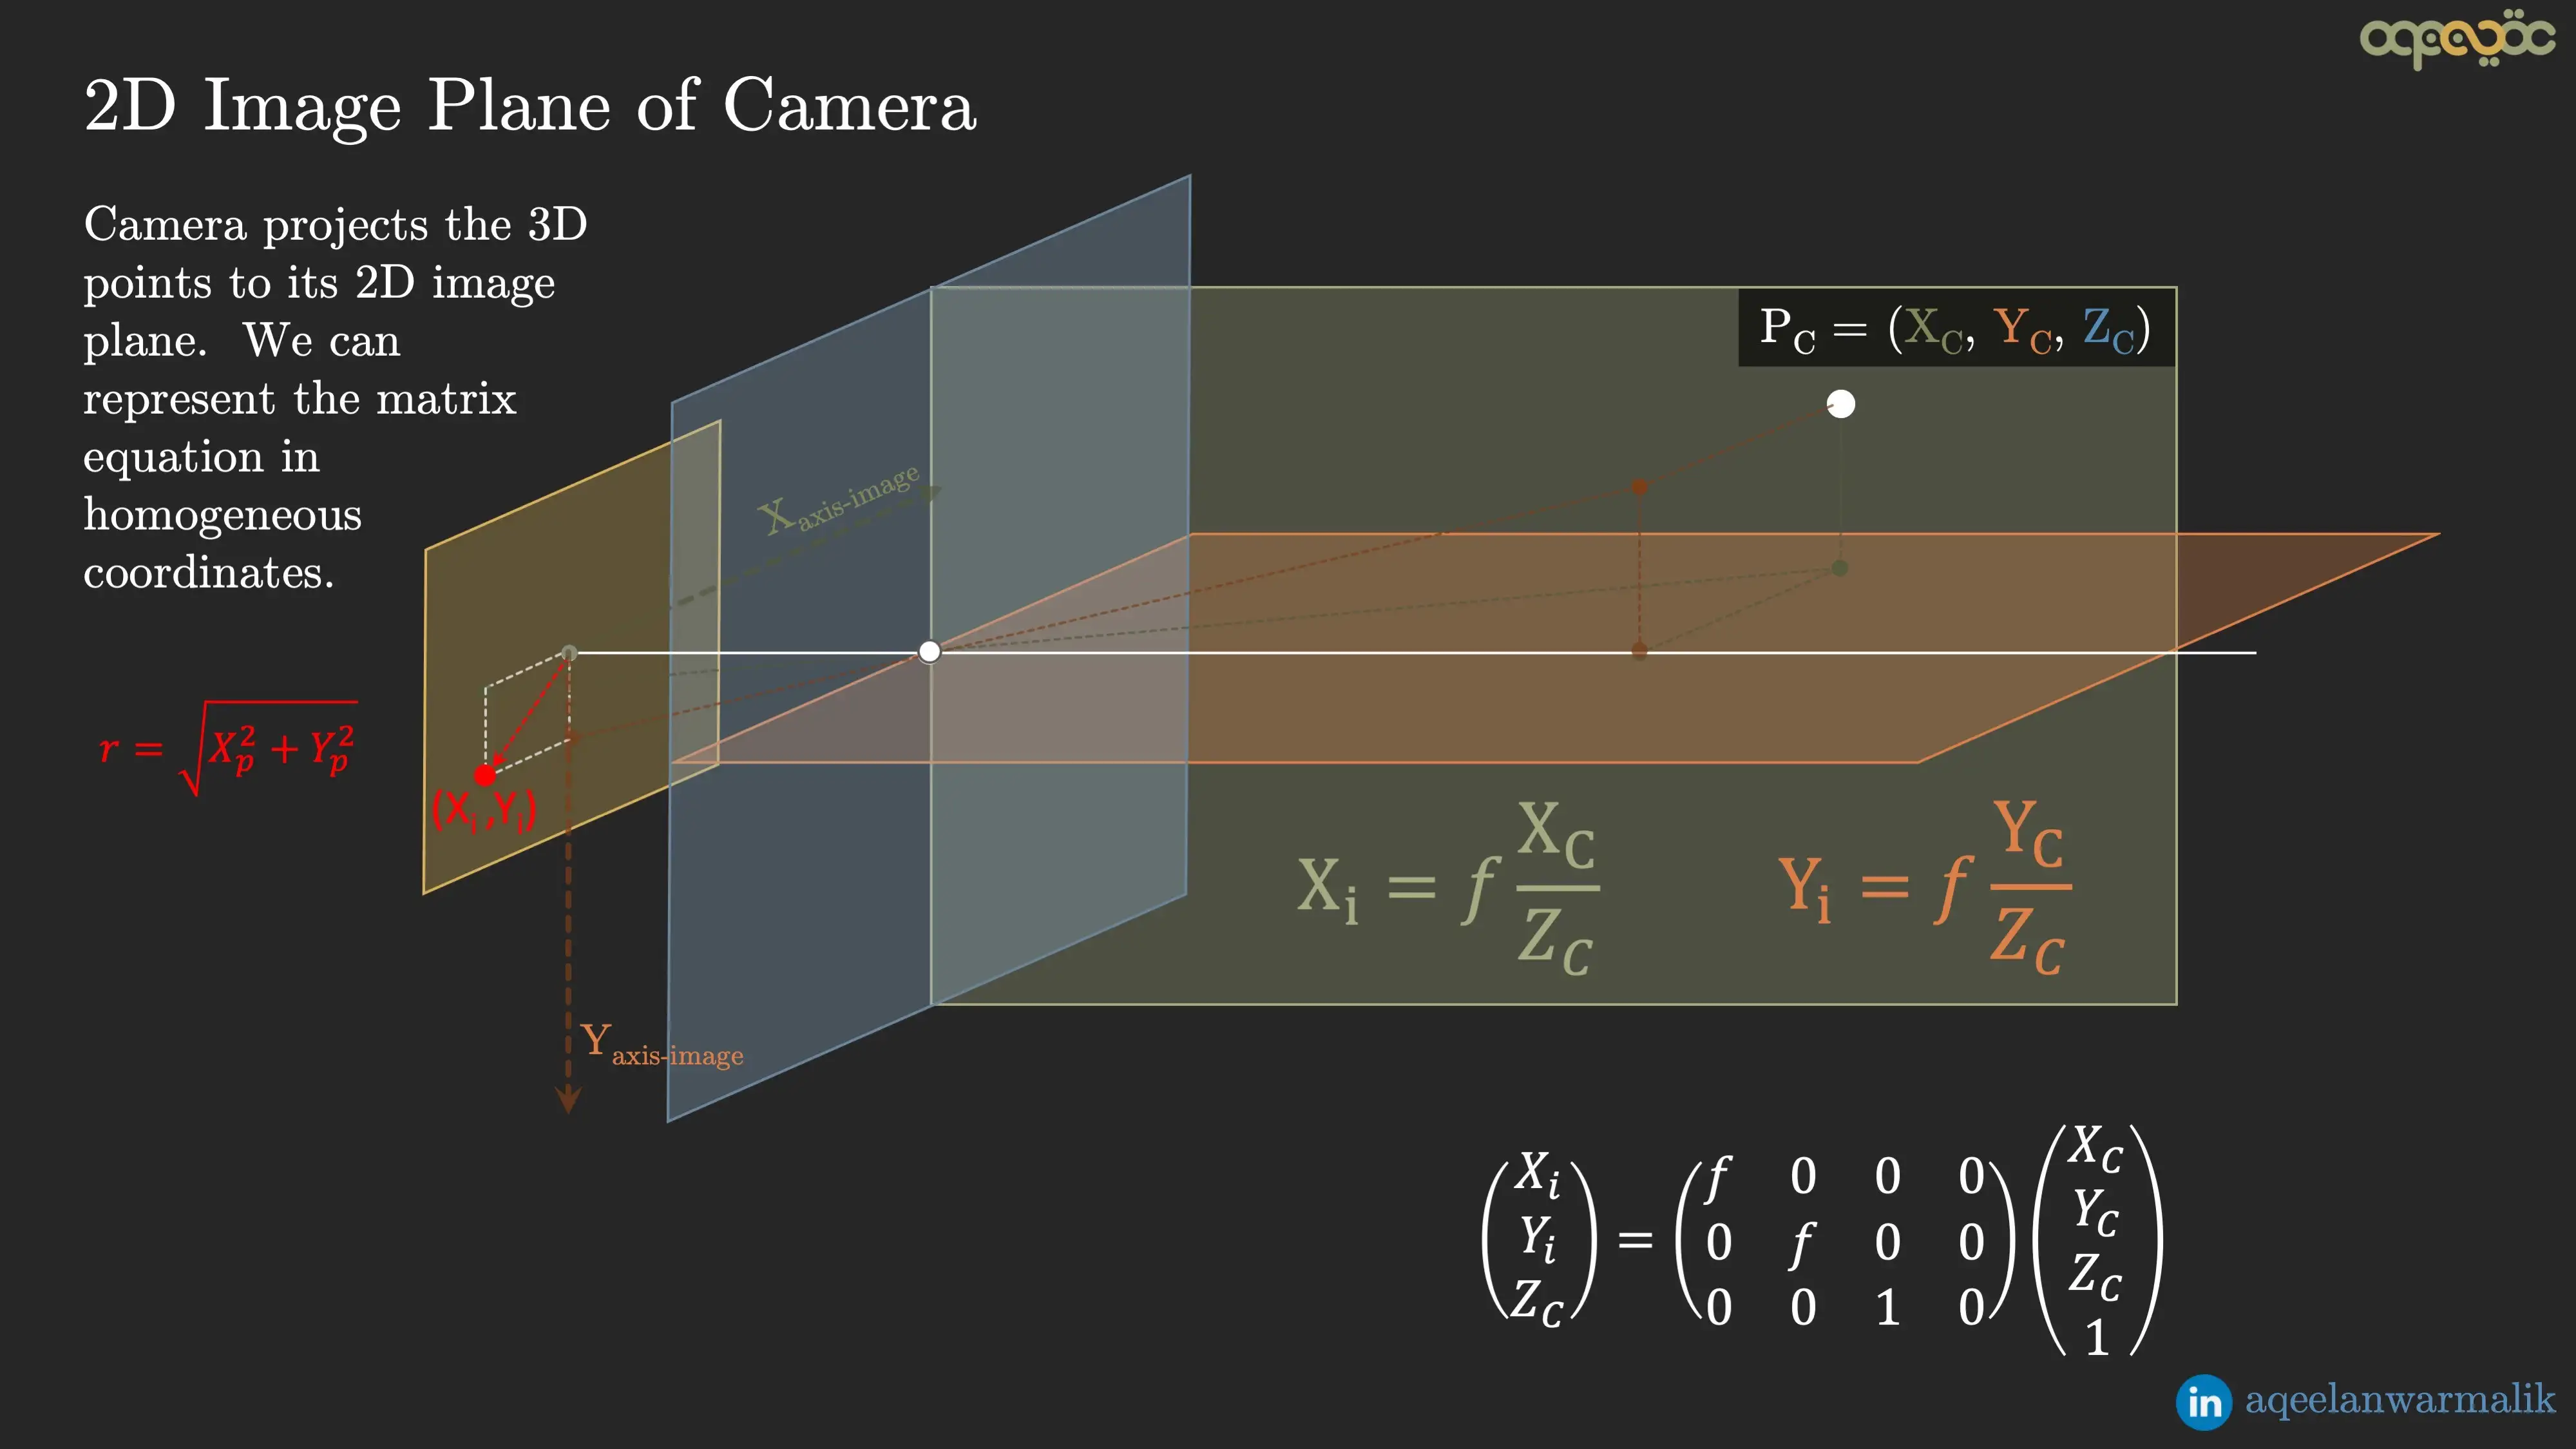
\includegraphics[scale=0.08]{img/int_matrix.png}
\end{center}
Now if there are distortions due to some lens on top of the pinhole, then this is when we would account for this. Usually, we account for a polynomial distortion, such as 
\begin{align*}
    x_{distorted} & = x (1 + k_1 r^2 + k_2 r^4 + k_3 r^6 ) \\
    y_{distorted} & = y (1 + k_1 r^2 + k_2 r^4 + k_3 r^6 )
\end{align*}
We will assume that there are no distortions, so working with $(x_i, y_i)$. Now if we discretize the $(x_i, y_i)$ to pixel coordinates $(u, v)$, then we can finally represent the points as an image matrix. Let us assume that the pixel coordinates of this image are discrete values, with $\rho_u$ pixels/meter in the $x$-axis and $\rho_v$ pixels/meter in the $y$-axis, so we first scale it. Since the origin of the image coordinates lie at the center of the image plane while the pixel coordinates has their origin defined at the top-left corner of the image, we should translate it by a certain $c_u$ and $c_v$ in the $x$ and $y$ axes. Therefore, we have 
\[\begin{cases} u & = \rho_u x_i + c_u \\ v & = \rho_V y_i + c_v \end{cases} \implies \begin{pmatrix} u \\ v \\ 1 \end{pmatrix} = \begin{pmatrix} \rho_u  & 0 & c_u \\ 0 & \rho_v & c_v \\ 0 & 0 & 1 \end{pmatrix} \begin{pmatrix} x_i \\ y_i \\ 1 \end{pmatrix}\]
Now this two-step process of projecting the image and discretizing it gives us the \textbf{camera intrinsic matrix}, defined 
\[\begin{pmatrix} \rho_u f z_C & 0 & c_u / z_C \\ 
0 & \rho_v f / z_C & c_v z_c & 0 \\ 
0 & 0 & 1/z_C & 0 \end{pmatrix} = \begin{pmatrix} \rho_u  & 0 & c_u \\ 0 & \rho_v & c_v \\ 0 & 0 & 1 \end{pmatrix} \begin{pmatrix} f/z_C & 0 & 0 & 0 \\ 0 & f/z_C & 0 & 0 \\ 0 & 0 & 1/z_C & 0 \end{pmatrix} \]
So, combining everything into one step, we have the equation 
\[\begin{pmatrix} u \\ v \\ 1 \end{pmatrix} = \underbrace{\begin{pmatrix} \rho_u f / z_C & 0 & c_u / z_C & 0\\ 
0 & \rho_v f / z_C & c_v / z_C & 0 \\ 
0 & 0 & 1/z_C & 0 \end{pmatrix}}_{\text{intrinsic}} \underbrace{\begin{pmatrix} \mathbf{R} & \mathbf{t} \\ \mathbf{0}^T & 1 \end{pmatrix}}_{\text{extrinsic}} \begin{pmatrix} x_W \\ y_W \\ z_W \\ 1 \end{pmatrix}\]
Sometimes, we write it by putting the $Z_C$ to the other side, and denoting it a constant $s$, which is the "hidden" scale factor representing depth. So, we have 
\[ s \begin{pmatrix} u \\ v \\ 1 \end{pmatrix} = \begin{pmatrix} \rho_u f & 0 & c_u & 0\\ 
0 & \rho_v f & c_v & 0 \\ 
0 & 0 & 1 & 0 \end{pmatrix} \begin{pmatrix} \mathbf{R} & \mathbf{t} \\ \mathbf{0}^T & 1 \end{pmatrix} \begin{pmatrix} x_W \\ y_W \\ z_W \\ 1 \end{pmatrix}\]
If two vectors are proportional in the sense that $\mathbf{v} = c \mathbf{u}$, then we write $\mathbf{u} \simeq \mathbf{v}$. So, we can write 
\[\begin{pmatrix} u \\ v \\ 1 \end{pmatrix} \simeq \begin{pmatrix} \rho_u f & 0 & c_u\\ 
0 & \rho_v f & c_v \\ 
0 & 0 & 1 \end{pmatrix} \big( \mathbf{R} \mathbf{p}_W + \mathbf{t} \big)\]

\section{Visual Intertial SLAM}

The input to a typical visual SLAM algorithm are a series of images (frames) captured from a camera. These would usually be RGB images, but with more advanced cameras (RGB-D or Opti-Track), they can accept more data. 
\begin{enumerate}
    \item \textbf{Tracking}: The tracking module detects feature points in the image (using feature detection algorithms such as SIFT, SURF, ORB) and uses them to find correspondences with a previous reference image, called a \textbf{keyframe}. Based on the correspondences, it simultaneously calculates the relative odometry between the reference keyframe and the current frame and calculates the map points, which can be thought of as the feature points reprojected into 3D space that help construct a map (feature points are in $\mathbb{R}^2$ and map points in $\mathbb{R}^3$, but they both essentially represent the same point). Then, the module determines if this frame should be added as another keyframe (based on a series of conditions s.t. its features can't be too similar or to different from the previous keyframe). If it does decide that this should be a keyframe, then it passes it to the local mapping module. In summary, this module does 3 things: 
    \begin{enumerate}
        \item It uses \textbf{visual odometry} to compute the ego-motion of the agent. It \textit{does not} build a map. 
        \item At the same time it extracts \textbf{map points}. A collection of feature points sounds like a map itself, but surprisingly, these map points are not used as inputs for the local mapping module that builds maps. It does sacrifice the computing efficiency by "throwing away" this calculation, but it does allow more parallelism due to executing the tracking, local mapping, and loop closing in separate threads. 
        \item It determines which keyframes should be used to build a map. 
    \end{enumerate}
    
    \item \textbf{Local Mapping}: This module creates correspondences between the new keyframe and other keyframes in the map. It then performs \textbf{bundle adjustment} through \textbf{Maximum a Posteriori (MAP)} estimation, a process of refining the relative coordinates of where the images were taken given the detected common features between keyframes. 
    
    \item \textbf{Loop Closing}: This new keyframe is compared to all other keyframes to check if the current location is the same as a previously visited location. If the current keyframe is similar to the previous one, this module will perform fusion of these keyframes and all related ones. It also performs pose optimization, typically as a \textbf{graph optimization}. Realistically, for computational reasons, this is done every once in a while rather than at every keyframe. 
\end{enumerate}
Note that to construct the global map, we basically take keyframes and the ego-motion between them. Essentially, a map is a graph where the vertices correspond to image frames, and edges correspond to 3D visual transformations between them. Ultimately, the agent records map points in a keyframe, then goes through some estimated motion, and then records map points in another keyframe, some of which may be the same points as before, and projects these points to $\mathbb{R}^3$ to construct the map. 

\subsection{Odometry: Keyframes and Map Points}

The image taken from a monocular camera is just a 2D projection of the 3D space. If we want to recover the 3D structure, we just have to change the camera's view angle. In monocular SLAM, we move the camera and estimate its motion, as well as the distances and sizes of the objects in the scene. From everyday experiences, we know that if we move to the right, everything in our frame moves to the left. Additionally, closer objects move faster, while farther objects move slower. Thus, when the camera moves, the movement of these obejcts on the image forms pixel disparity, which can be used to quantitatively determine the depth of various objects. But these are all relative values; we don't know the actual size of these objects. 

Stereo cameras consist of two synchronized monocular cameras, displaced with a known distance, called the \textbf{baseline}. Because the physical distance of the baseline is known, we can take the two frames captured at the same moment and use the differences between the images to calculate the depth. Usually, the further the baseline, the more reliable for further distances. 

Let us assume that we are working with monocular cameras with pinhole lens. If we have a camera which takes a frame, then moves, and then takes another frame, we can estimate the ego-motion of the camera and the map points with the following visual. 
\begin{center}
    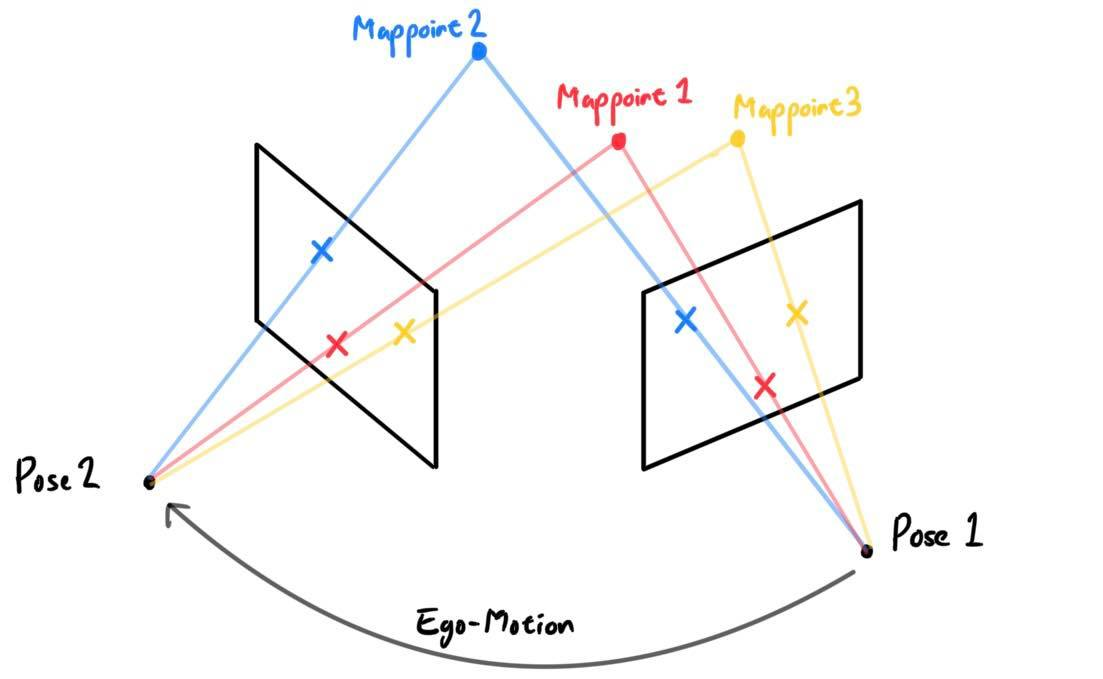
\includegraphics[scale=0.23]{img/visual_odometry.jpg}
\end{center}
Given that you know the two poses, you can "project" them out to 3D space to estimate the map points, and given that you know the map points, you can use the differences in the feature points between the frames to estimate the pose. This is sort of a chicken-or-egg scenario, which is why this is called simultaneous localization and mapping. Fortunately, due to the \textbf{8-point algorithm}, if we can find at least 8 common feature points between 2 frames, we can estimate the camera pose and map point position (since knowing one leads to the other). Furthermore, in visual-inertial SLAM, we have the inertial measurements from the IMU, too. For example, since it measures linear acceleration $\mathbf{a}$, we can integrate it twice to get the linear displacement: 
\[\Delta \mathbf{x} = \iint \mathbf{a}\,dt\]
and optimize this noisy estimate with the 8-point algorithm. Note that the 8-point algorithm is used in odometry and not in local mapping. 

Mathematically, visual-inertial odometry is a function that takes in a series of frames (which can really be stripped down to their sets of feature points) and the inertial inputs (from the IMUs). It outputs the ego-motion of the agent between the frames, which is some element $\phi \in \mathrm{SE}(3)$, a set of keyframes, and a set of map points. The important part is the $\phi$'s, which encode the localization information and thus gives us a rough pose of the camera. 
A key difference between odometry and map building is that odometry takes in \textit{every} frame to determine ego-motion, localization, and map points, while local mapping uses only keyframes to construct maps. In odometry, we could compare adjacent frames $v_{k}, v_{k+1}$, but it is generally preferred to compare a frame to the latest keyframe (since these are considered more optimized and stable). 
\begin{center}
    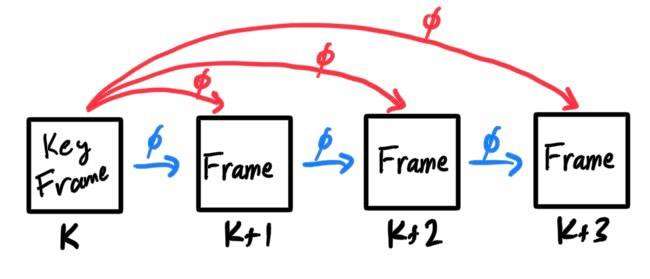
\includegraphics[scale=0.3]{img/VO_comparison.jpg}
\end{center}
These keyframes are then sent to the local mapping module, which creates \textit{new} 3D map points via triangulation. An optimized camera pose can be then calculated by solving the bundle adjustment problem, ultimately creating a global map (along with outputting the trajectory of the camera). 

\subsection{Local Mapping: Bundle Adjustment}

Geometric BA that minimizes feature reprojection error, or photometric BA that minimizes the photometric error of a set of selected pixels. Global vs local bundle adjustment. 

\subsection{Loop Closing}

\subsection{Mathematical Formulation of SLAM}

Now that we have some qualitative understanding of SLAM, along with some of the mathematical machinery for it, let us explain the problems we're trying to solve. We can model this using a discrete time model since the camera frames are coming in discrete moments. 
\begin{enumerate}
    \item Let the camera/agent have poses $\mathbf{x}_1, \ldots, \mathbf{x}_K$ (composed of both location and orientation). 
    \item Assume that the map is made up of several \textit{landmarks} $\mathbf{y}_1, \ldots, \mathbf{y}_N$. 
    \item At each timestep, we can use input commands $\mathbf{u}_{k-1}$ to direct the agent (e.g. turn 15 degrees to the left). That is, given command $\mathbf{u}_k$, we expect $\mathbf{x}_{k-1}$ to go to $\mathbf{x}_{k}$, with some additional noise $\mathbf{w}_k$. This function $f$ is called the \textbf{motion equation}. 
    \[\mathbf{x}_{k} = f(\mathbf{x}_{k-1}, \mathbf{u}_k) + \mathbf{w}_k\]
    This represents the localization portion of SLAM, and the notation is consistent with the robotics. For example, we can think of the pose as a 6-DoF element $\mathbf{x}_{k-1} \in \mathrm{SE}(3)$, the command $\mathbf{u}_k$ would also be an element of $\mathrm{SE}(3)$ representing some transformation, and the function $h: \mathrm{SE}(3) \times \mathbf{SE}(3) \longrightarrow \mathrm{SE}(3)$ is simply the group operator (matrix multiplication). There are many different representations of this. 
    
    \item Along with the motion equation, we have a \textbf{observation equation} that describes the process that the agent spots landmark $\mathbf{y}_j$ at pose $\mathbf{x}_k$, and generates some observation data $\mathbf{z}_{k, j}$. We can describe this relationship with some abstract function $h$. 
    \[\mathbf{z}_{k, j} = h (\mathbf{y}_j , \mathbf{x}_k) + \mathbf{v}_{k, j}\]
    This represents the mapping portion of SLAM. More specifically, $\mathbf{x}_k \in \mathrm{SE}(3)$ describes the pose of the agent in world coordinates, and the landmark/mappoint $\mathbf{y}_j \in \mathbb{R}^3$ is just some point. The pose $\mathbf{x}_k$ will determine where the agent is facing and where it can view, and the function $h$ will project all $\mathbf{r}_j$ to image coordinates $\mathbf{z}_{k, j} \in \mathbb{R}^2$ for all $k, j$. Say that at pose $\mathbf{x}_k$, the camera can see $\mathbf{y}_1$ in its view. Then, $h(\mathbf{y}_1, \mathbf{x}_k)$ will end up being the projection of $\mathbf{y}_1 \in \mathbb{R}^3$ in the world coordinates to $\mathbf{z}_{k, 1} \in \mathbb{R}^2$ in the image coordinates (so $h$ can be thought of as the extrinsic matrix followed by intrinsic matrix multiplication). If $\mathbf{y}_2$ is not visible, it will return a null value. 
\end{enumerate}
So, our model consists of two stochastic processes: 
\begin{align*}
    \mathbf{x}_{k} & = f(\mathbf{x}_{k-1}, \mathbf{u}_k) + \mathbf{w}_k \\
    \mathbf{z}_{k, j} & = h (\mathbf{y}_j , \mathbf{x}_k) + \mathbf{v}_{k, j}
\end{align*}
Now we assume that the noise are Gaussian: $\mathbf{w}_k \sim \mathcal{N}(\mathbf{0}, \mathbf{R}_k)$ and $\mathbf{v}_{k, j} \sim \mathcal{N}(\mathbf{0}, \mathbf{Q}_{k, j})$. 

For better visualization, at each time $k = 1, \ldots, K$, we have the following. At $k = 0$, we know the initial $\mathbf{x}_0$, and we give the command $\mathbf{u}_1$, which gives us $\mathbf{x}_1$. At this point, we want to take all map points $\mathbf{y}_j$ and compute its image coordinates, which can give some successful coordinates (if the mappoints are within the frame) and some null. 
\begin{center}
    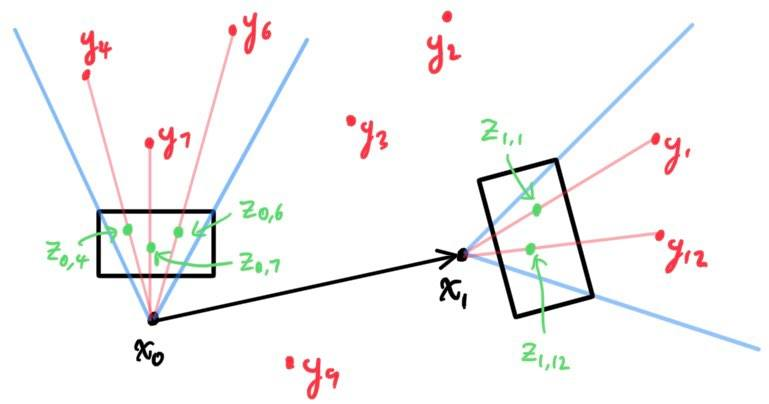
\includegraphics[scale=0.4]{img/time_1.jpg}
\end{center}
We may get some results at timestep $1$ such as 
\[\mathbf{z}_{1, 1} = \begin{pmatrix} 13 \\ 340 \end{pmatrix} , \; \mathbf{z}_{1, 2} = \emptyset, \ldots \]
So after all timesteps, we would have to keep track of the following: 
\begin{enumerate}
    \item The $K$ poses, which are all stochastic
    \[\mathbf{x} = \{\mathbf{x}_0, \mathbf{x}_1, \mathbf{x}_2, \ldots, \mathbf{x}_K\}\]
    where $\mathbf{x}_0$ is known. 
    \item The $N$ landmarks, which are all known in world coordinates, 
    \[\mathbf{y} = \{ \mathbf{y}_1, \ldots, \mathbf{y}_N\}\]
    
    \item The $K$ input commands, which are all known
    \[\mathbf{u} = \{\mathbf{u}_1, \ldots, \mathbf{u}_K\}\]
    
    \item The $N$ $2$-vectors at each time step $k \in [K]$, 
    \[\mathbf{z} = \{\mathbf{z}_1, \ldots, \mathbf{z}_K\}, \text{ where } \mathbf{z}_k = \begin{pmatrix} \mathbf{z}_{1, 1} \in \mathbb{R}^2 \\ \vdots \\ \mathbf{z}_{1, N} \in \mathbb{R}^2 \end{pmatrix} \]
\end{enumerate}

Since this data comes gradually over time, we can hold an estimated state at the current moment and then update it with new data. This method is called \textbf{filtering}. However, this method is outdated (20+ years old). A more modern way is to record the data into a file an look for the best trajectory and map in \textit{all} time, which is commonly known as \textbf{batch estimation}. 

Note that we completely know our input commands $\mathbf{u}_k$, along with the outputs $\mathbf{z}_{k, n}$ representing the image coordinates of the $N$ landmarks at each pose. From this data, we must infer the actual poses $\mathbf{x}$ and the landmark positions $\mathbf{y}$, which can be fully represented by the conditional probability distribution: 
\[P(\mathbf{x}, \mathbf{y} \mid \mathbf{u}, \mathbf{z}) \propto P(\mathbf{z}, \mathbf{u} \mid \mathbf{x}, \mathbf{y}) \; P (\mathbf{x}, \mathbf{y})\]
Note that this is a posterior distribution over \textit{all} $K$ poses and $N$ landmarks, i.e. this is a probability measure over the space 
\[\mathrm{SE}(3)^K \times (\mathbb{R}^3)^N\]
It is quite hard to find this posterior in nonlinear systems (which is what we will be working with), but it is feasible to optimize it, i.e. find the mode. 
\[(\mathbf{x}, \mathbf{y})^*_{MAP} = \arg \max P(\mathbf{x}, \mathbf{y} \mid \mathbf{z}, \mathbf{u}) = \arg \max P(\mathbf{z}, \mathbf{u} \mid \mathbf{x}, \mathbf{y}) \; P(\mathbf{x}, \mathbf{y})\]
If we take an improper prior, we can just solve the \textbf{Maximum Likelihood Estimation} 
\[(\mathbf{x}, \mathbf{y})^*_{MLE} = \arg \max P(\mathbf{z}, \mathbf{u} \mid \mathbf{x}, \mathbf{y})\]


\section{Visual Odometry}

\subsection{Feature Mapping: ORB}

Remember that if we would like to compute the ego-motion of our agent, it is more efficient to extract feature points from our frames to reduce the dimensionality of our problem. Extracting these feature points is extremely important since they determine the quality of our data. Ideally, we want feature points to remain stable after the camera moves, and when the scene/angle view changes slightly, the algorithm can determine from the iamges which places refer to the same point. Furthermore, we would want these feature points to be rotation and scale invariant, since that shouldn't affect which points are important. Therefore, we may use some radially symmetric kernel to detect keypoints. For simple algorithms, we can look at a grayscale image, but for most modern ones, the gray value alone is not feasible.


A feature point is composed of two parts: 
\begin{enumerate}
    \item A \textbf{key point}, which is the 2D position of the feature point in an image. 
    \item A \textbf{descriptor} is usually a vector describing the information of the pixels around the key point and used for identifying the same object in multiple key points. Features with similar appearance should have similar descriptors that are close within their vector space, and this metric can be used for feature mapping. Usually, the L2 Euclidean distance is used, and for binary descriptors (BRIEF), the Hamming distance is used. As the number of dimensions increases, we must also use approximate nearest neighbor searches. 
\end{enumerate}

The SIFT (Scale Invariant Feature Transform) is one of the most accurate and robust (through different angles, perspectives, and lighting changes), but it is extremely expensive. The FAST algorithm exchanges accuracy and robustness for calculation speed increase, and only calculates the keypoint (not the descriptor). The ORB (Oriented FAST and Rotated BRIEF) algorithm is widely used for real-time image feature extraction. To compare performance, extracting about 1000 feature points in the same image takes about 15.3 ms for ORB, 217.3ms for SURF, and 5228.7ms for SIFT. Big differences. 

Learning about each algorithm is beyond the scope of this course, so we will learn about the ORB feature. They consist of two parts: \textbf{ORB key points} and \textbf{ORB descriptors}. 
\begin{enumerate}
    \item FAST corner point extraction basically finds the corner points in the images and computes the main direction of the feature points, making the BRIEF descriptor rotation invariant. 
    \item The BRIEF descriptor describes the surrounding image area where the feature points were extracted in the previous step. ORB 
\end{enumerate}

\subsubsection{FAST Key Point}
We take a grayscale image and do the following: 
\begin{enumerate}
    \item Select pixel $p$ from the image, assuming its brightness as $I_p$. 
    \item Set a threshold $T$, for example $20\%$ of $I_p$. 
    \item Take $p$ as center, and select the 16 pixels on a circle with a radius of $3$. 
    \item If there are consecutive $N$ points on the selected circle whose brightness is outside of $[I_p - T, I_p + T]$, then $p$ can be considered a feature point. $N = 12$ usually: FAST-12. 
    \item Iterate through the above 4 steps with each pixel. 
\end{enumerate}
There are some optimization techniques but this algorithm suffers from lousy repeatability and uneven distribution. Another problem is that the original FAST corners are often clustered. 

Furthermore, because it fixed the radius of the circle as $3$, there is also a scaling problem: a place that looks like a corner from a distance may not be a corner when it comes close. This is solved by an image pyramid. The bottom of the pyramid is the original image, and for each layer up, the image is scaled to produce different resolutions. The smaller image can be seen as a scene viewed from a distance. We can match images on different layers to achieve scale invariance. 

Finally, let us talk about rotation invariance. To know this, we must define the centroid of an image. Given an image block $B$ consisting of pixels $(x, y)$ with their grayscale intensities $I(x, y)$, let us define the \textbf{moment} of the image block $B$ as 
\[M_{p q} \coloneqq \sum_{(x, y) \in B} x^p y^q \, I(x, y)\]
Then, the \textbf{centroid} of $B$ is defined 
\[C = \bigg(\frac{m_{10}}{m_{00}} , \frac{m_{01}}{m_{00}} \bigg)\]
Connect the geometric center $O$ and the centroid $C$ of the image block to get an direction vector $\overrightarrow{OC}$, so the direction of the feature point can be defined as 
\[\theta = \mathrm{arctan}\Big( \frac{m_{01}}{m_{10}} \Big)\]
With this information, we can improve the feature points to be rotation invariant, thus resulting in Oriented FAST. 

\subsubsection{BRIEF Descriptor and Feature Matching}
BRIEF is a binary descriptor that encodes the size relationship between 2 random pixels $p$ and $q$ near the key point. If $I_p > I_q$, then take $1$, and $0$ otherwise. If we take $n$ such pairs, we get a $n$-dimensional vector in $\{0, 1\}^n$. This BRIEF algorithm implements the comparison of randomly selected points, which is very fast. 

Now we can calculate (using the Hamming distance) between the BRIEF descriptors to determine which key points match the same object. However, mismatches are common due to the locality of image features. Due to repeated textures in the scene, feature descriptions can be very similar, so it is hard to resolve this mismatch by using local features only. The most naive is the brute force method: Assume features $x_t^m$, $m =1, \ldots M$ are extracted in image $I_t$ and features $x_{t+1}^n$, $n = 1, \ldots, N$ in image $I_{t+1}$. We can just brute force this by computing the $M N / 2$ distances and then sorting. But this is not computationally efficient, which is why we can use more sophisticated methods, such as the Fast Approximate Nearest Neighbor (FLANN) algorithm. The technical details will be skipped here, but here are two pictures with points that have been feature matched. 
\begin{center}
    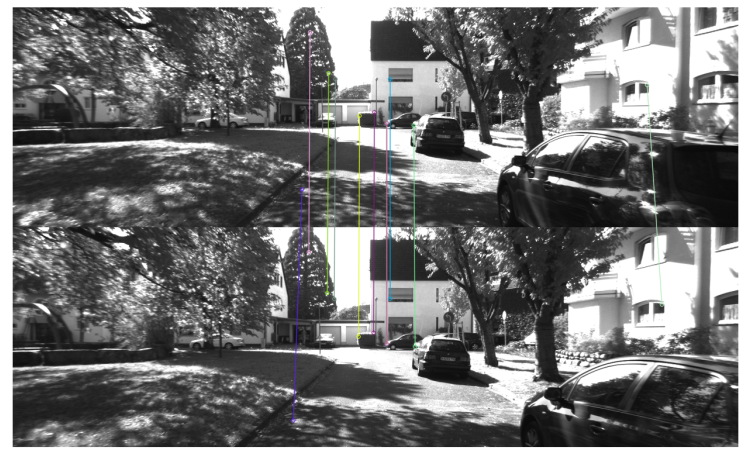
\includegraphics[scale=0.4]{img/feature_matching.png}
\end{center}

\subsection{2D-2D Epipolar Geometry: Estimating Ego-Motion}

\begin{center}
    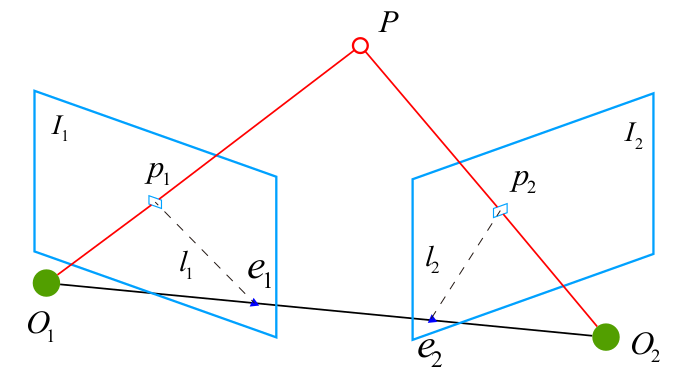
\includegraphics[scale=0.35]{img/epipolar_geometry.png}
\end{center}

We will refer to the diagram above. Let's have some map point in world coordinates $\mathbf{p}_W = (x_W, y_W, z_W)^T$. Let the camera position $C_1$ be represented by $\mathbf{R}_1$ and $\mathbf{t}_1$, and that of $C_2$ be represented by $\mathbf{R}_2$ and $\mathbf{t}_2$. Then, we can represent the camera coordinates as 
\begin{align*}
    \begin{pmatrix} \mathbf{p}_{C_1} \\ 1 \end{pmatrix} & = \begin{pmatrix} \mathbf{R}_1 & \mathbf{t}_1 \\ \mathbf{0}^T & \mathbf{1} \end{pmatrix} \begin{pmatrix} \mathbf{p}_W \\ \mathbf{1} \end{pmatrix} \\ 
    \begin{pmatrix} \mathbf{p}_{C_2} \\ 1 \end{pmatrix} & = \begin{pmatrix} \mathbf{R}_2 & \mathbf{t}_2 \\ \mathbf{0}^T & \mathbf{1} \end{pmatrix} \begin{pmatrix} \mathbf{p}_W \\ \mathbf{1} \end{pmatrix} \\
    & = \begin{pmatrix} \mathbf{R}_{21} & \mathbf{t}_{21} \\ \mathbf{0}^T & \mathbf{1} \end{pmatrix} \begin{pmatrix} \mathbf{R}_1 & \mathbf{t} \\ \mathbf{0}^T & \mathbf{1} \end{pmatrix} \begin{pmatrix} \mathbf{p}_W \\ \mathbf{1} \end{pmatrix} \\
    & = \begin{pmatrix} \mathbf{R}_{21} & \mathbf{t}_{21} \\ \mathbf{0}^T & \mathbf{1} \end{pmatrix} \begin{pmatrix} \mathbf{p}_{C_1} \\ 1 \end{pmatrix}
\end{align*} 
From our previous notation, we know that the intrinsic camera matrix has dimensions $\mathbf{K} \in \mathbb{R}^{3 \times 4}$ that maps from the homoegenous 3D coordinates to homogeneous 2D coordinates. We can also write 
\begin{align*}
    \mathbf{p}_{C_1} & = \mathbf{R}_1 \mathbf{p}_W + \mathbf{t}_1 \\ 
    \mathbf{p}_{C_2} & = \mathbf{R}_{21} \mathbf{p}_{C_1} + \mathbf{t}_{21}
\end{align*}
We can work with 3D camera coordinates $(x, y, z)$ and stick with the 3D homogeneous image coordinates $(u, v, 1)$. Then, our intrinsic matrix is the previous one with the rightmost column truncated, which will be denoted $\mathbf{K}$ from now on. 
\[s \mathbf{u} = s \begin{pmatrix} u \\ v \\ 1 \end{pmatrix} = \begin{pmatrix} \rho_u f & 0 & c_v \\ 0 & \rho_v f & c_v \\ 0 & 0 & 1 \end{pmatrix} \mathbf{p}_C\]
Then, we can write the image projections of $\mathbf{p}_W$ onto each camera frame as $s_1 \mathbf{u}_1 = \mathbf{K} \mathbf{p}_{C_1}$ and $s_2 \mathbf{u}_2 = \mathbf{K} (\mathbf{R} \mathbf{p}_{C_1} + \mathbf{t})$. Since $K$ is invertible (upper diagonal with nonzero product of diagonal entries), we can define $\mathbf{x}_1 = \mathbf{K}^{-1} \mathbf{u}_1$ and $\mathbf{x}_2 = \mathbf{K}^{-1} \mathbf{u}_2$. 
\begin{align*}
    \mathbf{x}_1 = \mathbf{K}^{-1} \mathbf{u}_1 & = \frac{1}{s_1} \mathbf{p}_{C_1} \\ 
    \mathbf{x}_2 = \mathbf{K}^{-1} \mathbf{u}_2 & = \frac{1}{s_2} \big( \mathbf{R} \mathbf{p}_{C_1} + \mathbf{t} \big) \\
    & = \frac{s_1}{s_2} \bigg( \frac{1}{s_1} \mathbf{R} \mathbf{p}_{C_1} + \frac{1}{s_1} \mathbf{t} \bigg) \\
    & = \frac{s_1}{s_2} \big( \mathbf{R} \mathbf{x}_1 + \frac{1}{s_1} \mathbf{t} \big) 
\end{align*}
Define 
\[\mathbf{t}^\wedge = \begin{pmatrix} 0 & -t_3 & t_2 \\ t_3 & 0 & -t_1 \\ -t_2 & t_1 & 0 \end{pmatrix}\]
We left multiply $\mathbf{x}_2^T \mathbf{t}^\wedge$ on both sides of the final line, which reduces the left side to $0$. 
\[0 = \mathbf{x}_2^T \mathbf{t}^\wedge \mathbf{x}_2 = \mathbf{x}_2^T \mathbf{t}^\wedge \bigg( \frac{s_1}{s_2} \big( \mathbf{R} \mathbf{x}_1 + \frac{1}{s_1} \mathbf{t} \big) \bigg) = \frac{s_1}{s_2} \mathbf{x}_2^T \mathbf{t}^\wedge \mathbf{R} \mathbf{x}_1\]
which gets us the \textbf{epipolar constraints}: 
\[\mathbf{x}_2^T \mathbf{t}^\wedge \mathbf{R} \mathbf{x}_1 = 0 \iff \mathbf{p}_2^T \mathbf{K}^{-T} \mathbf{t}^\wedge \mathbf{R} \mathbf{K}^{-1} \mathbf{p}_1 = 0\]
Geometrically, it means that $O_1, P, O_2$ are coplanar (obvious?). This constraint encodes both translation and rotation. 
\begin{enumerate}
    \item The \textbf{essential matrix} is defined $\mathbf{E} = \mathbf{t}^\wedge \mathbf{R}$. 
    \item The \textbf{fundamental matrix} is defined $\mathbf{F} = \mathbf{K}^{-T} \mathbf{E} \mathbf{K}^{-1}$. 
\end{enumerate}
This allows us to write 
\[\mathbf{x}_2 \mathbf{E} \mathbf{x}_1 = \mathbf{p}_2 \mathbf{F} \mathbf{p}_1 = 0\]
which shows the relationship between two matching points concisely. Therefore, based on the pixel positions of these mached points, we should first find $\mathbf{E}$ or $\mathbf{F}$, and then find $\mathbf{R}, \mathbf{t}$. Often the simpler form $\mathbf{E}$ is used in practice. It has the following properties: 
\begin{enumerate}
    \item Equivalence under different scales: Multiplying $\mathbf{E}$ by a different scale gives the same constraint. 
    \item The singular values of the $\mathbf{E}$ must be of form $(\sigma, \sigma, 0)$. 
\end{enumerate}
It turns out that the set of essential matrices form a 5-dimensional projective space. The fact that it has 5 DoF indicates that we can use at least 5 pairs of (nonredundant) points to solve $\mathbf{E}$. However, due to the nonlinearity of this space, we must use 8 pairs, which is the classical 8-point algorithm. 

\subsubsection{8-Point Algorithm}

Let's describe the algorithm. Consider a pair of matched points, with coordinates $\mathbf{u}_1 = (u_1, v_1, 1)^T$ and $\mathbf{u}_2 = (u_2, v_2, 1)^T$. We have 
\[\begin{pmatrix} u_2 & v_2 & 1 \end{pmatrix} \begin{pmatrix} e_1 & e_2 & e_3 \\ e_4 & e_5 & e_6 \\ e_7 & e_8 & e_9 \end{pmatrix} \begin{pmatrix} u_1 \\ v_1 \\ 1 \end{pmatrix} = 0\]
We rewrite the matrix in vector form $\mathbf{e} = (e_1, \ldots, e_9)^T$. Then, the epipolar constraint can be written in a linear form w.r.t. $\mathbf{e}$. 
\[\big( u_2 u_1 , u_2 v_1 , u_2 , v_2 u_1, v_2 v_1, v_2, u_1, v_1, 1 \big) \cdot \mathbf{e} = 0\]
Given that we have $8$ pairs of matched features $(\mathbf{u}^k, \mathbf{v}^k\}_{k=1}^8$, we can solve the linear system of equations
\[\begin{pmatrix} 
u_2^1 u_1^1 & u_2^1 v_1^1 & u_2^1 & v_2^1 u_1^1 & v_2^1 v_1^1 & v_2^1 & u_1^1 & v_1^1 & 1 \\
u_2^2 u_1^2 & u_2^2 v_1^2 & u_2^2 & v_2^2 u_1^2 & v_2^2 v_1^2 & v_2^2 & u_1^2 & v_1^2 & 1 \\
\vdots & \vdots & \vdots & \vdots & \vdots & \vdots & \vdots & \vdots & \vdots \\
u_2^8 u_1^8 & u_2^8 v_1^8 & u_2^8 & v_2^8 u_1^8 & v_2^8 v_1^8 & v_2^8 & u_1^8 & v_1^8 & 1 \end{pmatrix} \begin{pmatrix} e_1 \\ e_2 \\ e_3 \\ e_4 \\ e_5 \\ e_6 \\ e_7 \\ e_8 \\ e_9 \end{pmatrix} = \mathbf{0}\]
$\mathbf{e}$ is located in the null space of this matrix. The rank of the coefficient matrix can be at most $8$, and by the rank-nullity theorem, if this is of full rank, then the null space is of dimension $1$. Considering the equivalence property of $\mathbf{E}$, this gives us a unique solution. 

If we get $N > 8$ pairs of features, then we can calculate a least-squares solution. We can define the $N \times 9$ matrix $\mathbf{A}$ of coefficients and then solve the least squares solution for 
\[\mathbf{A} \mathbf{e} = \mathbf{0}\]
Now we must talk about how to retrieve $\mathbf{R}, \mathbf{t}$ from $\mathbf{E}$. We will skip technalities and just say that this can be solved by taking the SVD of $\mathbf{E} = \mathbf{U} \mathbf{\Sigma} \mathbf{V}^T$. 

\subsection{Triangulation: Estimating Map Points}

The first thing to note is that triangulation is caused by translation. Only when there is enough amount of translation, triangles in epipolar geometry can be formed, and then triangulation can be implemented. Therefore, triangulation cannot be used for pure rotation because the triangle does not exist in this case. We will refer to the diagram below. 

\begin{center}
    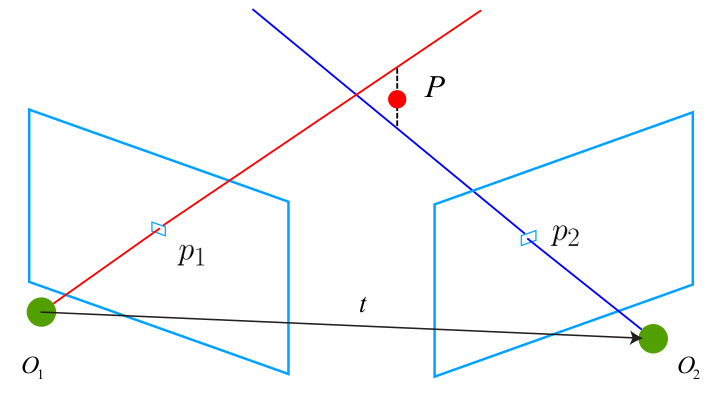
\includegraphics[scale=0.35]{img/triangulation.png}
\end{center}

Now given the matched features points, we have computed an estimate of $\mathbf{R}$ and $\mathbf{t}$. Now, we must still compute the depth of the mappoint $\mathbf{p}_W$ from $C_1$ and $C_2$, i.e. the variables $s_1$ and $s_2$. Remember that we have the projected image coordinates $\mathbf{u}_1, \mathbf{u}_2$ satisfying $s_1 \mathbf{u}_1 = \mathbf{K} \mathbf{p}_{C_1}$ and $s_2 \mathbf{u}_2 = \mathbf{K} (\mathbf{R} \mathbf{p}_{C_1} + \mathbf{t})$. By substituting, we get $s_1 \mathbf{x}_1 = \mathbf{p}_{C_1}$ and $s_2 \mathbf{x}_2 = \mathbf{p}_{C_2}$, i.e. we can interpret the $\mathbf{x}$'s as the normalized coordinates of $\mathbf{p}_C$. They satisfy 
\[s_2 \mathbf{x}_2 = s_1 \mathbf{R} \mathbf{x}_1 + \mathbf{t}\]
Geometrically, we want to find a 3D point on the ray $\overrightarrow{O_1 p_1}$ to make its projection as close to $\mathbf{p}_2$, same for the other point. Either way, the answer is similar. To estimate $s_1$, we can multiply both sides of the formula by $\mathbf{x}_2^\wedge$ to get 
\[0 = s_2 \mathbf{x}_2^\wedge \mathbf{x}_2 = \mathbf{s}_1 \mathbf{x}_2^\wedge \mathbf{R} \mathbf{x}_1 + \mathbf{x}_2^\wedge \mathbf{t}\]
With $s_1$, $s_2$ is easy to calculate, and we find their depth, multiply it by $\mathbf{x}_1, \mathbf{x}_2$, and find their spatial coordinates. Other more effective methods might be optimizing a least square cost function rather than directly solving it. 

\subsection{2D Optical Flow}


\subsection{Direct Method}



\section{Filters}

Note from before that we are trying to solve the equations 
\begin{align*}
    \mathbf{x}_{k} & = f(\mathbf{x}_{k-1}, \mathbf{u}_k) + \mathbf{w}_k \\
    \mathbf{z}_{k, j} & = h (\mathbf{y}_j , \mathbf{x}_k) + \mathbf{v}_{k, j}
\end{align*}
for $t = 0, \ldots, N$ and landmarks $m = 1, \ldots, M$. We would like to infer the values of $\mathbf{x}, \mathbf{y}$ using our values of $\mathbf{u}$ and $\mathbf{z}$. Due to noise, we know that these are random variables. For convenience of notation, let us denote all of our unknowns at time $t = k$ to be
\[\mathbf{X}_{k} \coloneqq \{\mathbf{x}_k, \mathbf{y}_1, \ldots, \mathbf{y}_M\}\]
We can also let $\mathbf{z}_k$ be the vector $(\mathbf{z}_{k, 1}, \mathbf{z}_{k, 2}, \ldots, \mathbf{z}_{k, M}$ and redefine $h$ as the vector-valued function that outputs the $\mathbf{z}_k$. So, our model looks like 
\begin{align*}
    \mathbf{X}_{k} & = f(\mathbf{X}_{k-1}, \mathbf{u}_k) + \mathbf{w}_k \\
    \mathbf{z}_{k} & = h (\mathbf{X}_k) + \mathbf{v}_{k}
\end{align*}

We would like to use the data from $1$ to $k$ to estimate the current state distribution $P (\mathbf{X}_k \mid \mathbf{X}_0, \mathbf{u}_{1:k}, \mathbf{z}_{1:k})$. Let us focus on the $\mathbf{z}_k$, which are the image points of all landmarks that we get for all timesteps so far. We can use Bayes' rule to expand 
\[P (\mathbf{X}_k \mid \mathbf{X}_0, \mathbf{u}_{1:k}, \mathbf{z}_{1:k}) \propto P(\mathbf{z}_k \mid \mathbf{X}_k) \; P(\mathbf{X}_k \mid \mathbf{X}_0, \mathbf{u}_{1:k}, \mathbf{z}_{1:k-1})\]
The likelihood tells us the probability of observing $\mathbf{z}_k$ given that we are at $\mathbf{X}_k$. We can condition over $\mathbf{X}_{k-1}$ on the prior since $\mathbf{X}_k$ must be dependent on $\mathbf{X}_{k-1}$. 
\[P(\mathbf{X}_k \mid \mathbf{X}_0, \mathbf{u}_{1:k}, \mathbf{z}_{1:k-1}) = \int P(\mathbf{X}_k \mid \mathbf{X}_{k-1}, \mathbf{X}_0, \mathbf{u}_{1:k}, \mathbf{z}_{1: k-1}) \; P (\mathbf{X}_{k-1} \mid \mathbf{X}_0, \mathbf{u}_{1:k}, \mathbf{z}_{1:k-1}) \; d \mathbf{X}_{k-1}\]
From here, we can make more assumptions for simplicity. 

\subsection{Linear Systems and the Kalman Filter}
We assume that $\mathbf{X}_k$ satisfies the Markov property, i.e. its state at $k$ is only affected by the state at $k-1$. So, we can get a recursive formula representing the state distribution of $\mathbf{X}_k$ ($P(\mathbf{X}_k \mid \mathbf{X}_0, \mathbf{u}_{1:k}, \mathbf{z}_{k-1})$) as something conditioned over the state distribution of $\mathbf{X}_{k-1}$ $P(\mathbf{X}_{k-1} \mid \mathbf{X}_0, \mathbf{u}_{1:k-1}, \mathbf{z}_{1:k-1})$. 
\[P(\mathbf{X}_k \mid \mathbf{X}_0, \mathbf{u}_{1:k}, \mathbf{z}_{1:k-1}) = \int P(\mathbf{X}_k \mid \mathbf{X}_{k-1}, \mathbf{u}_{k}) \; P (\mathbf{X}_{k-1} \mid \mathbf{X}_0, \mathbf{u}_{1:k-1}, \mathbf{z}_{1:k-1}) \; d \mathbf{X}_{k-1}\]
Since we assumed Gaussian noise, we know that all these random vectors $\mathbf{X}_1, \ldots, \mathbf{X}_k$ are Gaussian, so we can work with their means and covariance matrices. Now let us assume another thing: our system is linear, so the equations are of the form 
\begin{align*}
    \mathbf{X}_{k} & = \mathbf{A}_k \mathbf{X}_{k-1} + \mathbf{u}_k + \mathbf{w}_k \\
    \mathbf{z}_{k} & = \mathbf{C}_k \mathbf{X}_k + \mathbf{v}_{k}
\end{align*}
with noise $\mathbf{w}_k \sim \mathcal{N}(0, \mathbf{R})$ and $\mathbf{v}_{k} \sim \mathbf{N}(0, \mathbf{Q})$, with subscripts removed for conciseness. Now, in order to calculate the posterior, we must calculate the likelihood and prior in here. 
\[P (\mathbf{X}_k \mid \mathbf{X}_0, \mathbf{u}_{1:k}, \mathbf{z}_{1:k}) \propto P(\mathbf{z}_k \mid \mathbf{X}_k) \; P(\mathbf{X}_k \mid \mathbf{X}_0, \mathbf{u}_{1:k}, \mathbf{z}_{1:k-1})\]
Due to the Markov property, we don't need to condition over it and can find it if we know the posterior distribution of $\hat{\mathbf{X}}_{k-1} \sim \mathcal{N}(\hat{\mathbf{X}}_{k-1}, \hat{\mathbf{P}}_{k-1})$. Let us use $\hat{\mathbf{X}}$ to represent the posterior of $\mathbf{X}$ and $\check{\mathbf{X}}$ for the prior. 
\begin{enumerate}
    \item \textbf{Prediction Step}: The prior can be calculated simply by transforming the posterior Gaussian $\hat{\mathbf{X}}_{k-1}$ under the linear transformation and adding the extra noise $\mathbf{w}_k$. This gives us the formula for the prior 
    \[P(\mathbf{X}_k \mid \mathbf{X}_0, \mathbf{u}_{1:k}, \mathbf{z}_{1:k-1}) = \mathcal{N}(\mathbf{A}_k \hat{\mathbf{X}}_{k-1} + \mathbf{u}_k, \mathbf{A}_k \hat{\mathbf{P}}_{k-1} \mathbf{A}_k^T + \mathbf{R})\]
    So, we have $\check{\mathbf{X}}_{k} \sim \mathcal{N}(\mathbf{A}_k \hat{\mathbf{X}}_{k-1} + \mathbf{u}_k, \mathbf{A}_k \hat{\mathbf{P}}_{k-1} \mathbf{A}_k^T + \mathbf{R})$. 
    \item \textbf{Update Step}: The likelihood can be computed very easily since we are fixing $\mathbf{X}_k$. 
    \[P(\mathbf{z}_k \mid \mathbf{x}_k) = \mathcal{N}(\mathbf{C}_k \mathbf{x}_k, \mathbf{Q})\]
    \item Multiplying these two Gaussian densities gives us the posterior $\mathcal{N}(\hat{\mathbf{x}}_k, \hat{\mathbf{P}}_k)$. The arithmetic is quite involved, so in summary, we first calculate the \textbf{Kalman gain}: 
    \[\mathbf{K} = \check{\mathbf{P}}_k \mathbf{C}_k^T ( \mathbf{C}_k \check{\mathbf{P}}_k \mathbf{C}_k^T + \mathbf{Q}_k)^{-1}\]
    \item This gives us the formula for the posterior: 
    \[P (\mathbf{X}_k \mid \mathbf{X}_0, \mathbf{u}_{1:k}, \mathbf{z}_{1:k}) = \mathcal{N} \big( \check{\mathbf{x}}_k + \mathbf{K}(\mathbf{z}_k - \mathbf{C}_k \mathbf{x}_k), (\mathbf{I} - \mathbf{K} \mathbf{C}_k ) \check{\mathbf{P}}_k \big)\]
\end{enumerate}

\subsection{Nonlinear Systems and the Extended Kalman Filter}

Usually, the motion and observation equations are nonlinear models, but we can simply take the first order Taylor expansion to approximate them as linear systems. Let the mean and covariance matrix at time $k - 1$ be $\hat{\mathbf{x}}_{k-1}$ and $\hat{\mathbf{P}}_{k-1}$. Then, we simply expand at $\hat{\mathbf{x}}_{k-1}$ on the motion equation: 
\begin{align*}
    \mathbf{X}_k & \approx f(\hat{\mathbf{X}}_{k-1}, \mathbf{u}_k) + \frac{\partial f}{\partial \mathbf{X}_{k-1}} \bigg|_{\hat{\mathbf{X}}_{k-1}} (\mathbf{X}_{k-1} - \hat{\mathbf{X}}_{k-1}) + \mathbf{w}_k \\
    & = f(\hat{\mathbf{X}}_{k-1}, \mathbf{u}_k) + \mathbf{F} (\mathbf{X}_{k-1} - \hat{\mathbf{X}}_{k-1}) + \mathbf{w}_k 
\end{align*}
where we denote the total derivative as $\mathbf{F}$. For the observation model, we can just take the total derivative at $\mathbf{X}_k$. 
\begin{align*}
    \mathbf{z}_k & \approx h(\mathbf{X}_k) + \frac{\partial h}{\partial \mathbf{X}_k} \bigg|_{\mathbf{X}_k} (\mathbf{x}_k - \mathbf{X}_k) + \mathbf{u}_k \\
    & = h(\mathbf{X}_k) + \mathbf{H} (\mathbf{x}_k - \mathbf{X}_k) + \mathbf{u}_k 
\end{align*}
where we denote the total derivative as $\mathbf{H}$. Then, we can summarize the algorithm in the following way: 
\begin{enumerate}
    \item The prediction step is 
    \[\check{\mathbf{X}}_k \sim \mathcal{N}\big( f( \hat{\mathbf{X}}_{k-1}, \mathbf{u}_k), \mathbf{F} \hat{\mathbf{P}}_{k-1} \mathbf{F}^T + \mathbf{R}_k)\]
    \item The likelihood is of form 
    \[P(\mathbf{z}_k \mid \mathbf{x}_k) = \mathcal{N}\big( h(\mathbf{x}_k + \mathbf{H}(\mathbf{x}_k - \mathbf{X}_k), \mathbf{Q}_k \big)\]
    \item We compute the Kalman gain 
    \[\mathbf{K}_k = \mathbf{P}_k \mathbf{H}^T ( \mathbf{H} \mathbf{P}_k \mathbf{H}^T + \mathbf{Q}_k)^{-1}\]
    \item The posterior can be written 
    \[\hat{\mathbf{X}}_k \sim \mathcal{N}\big( \mathbf{X}_k + \mathbf{K}_k (\mathbf{z}_k - h(\mathbf{X}_k)), (\mathbf{I} - \mathbf{K}_k \mathbf{H}) \mathbf{P}_k \big) \]
\end{enumerate}

To describe the EKF, this is quite a simple algorithm that can be used to estimate the amount of uncertainty within a certain period of time in a lot of applications. However, EKF falls short in many aspects. First, the Markov property is too strong of an assumption, since a robot can be programmed to return the to starting position after a long time. The linearization can approximate quite badly, since for every step, the model is linearized only once. Finally, filter methods have no outlier detection mechanism, which causes the system to diverge when there are outliers. 

\section{Bundle Adjustment and Graph Optimization}
Bundle adjustment refers to optimizing both camera parameters (both intrinsic and extrinsic) and 3D landmarks with images. To put simply, consider the bundles of light rays emitted from 3D points. They are projected into the image planes of several cameras and then detected as feature points. The purpose of optimization can be explained as to adjust the camera poses and the 3D points, to ensure the projected 2D features (bundles) match the detected results. 

Recall the observation equation $\mathbf{z}_{i, j} = h(\mathbf{x}_i, \mathbf{y}_{j})$. So given a data point $\mathbf{z}_{i, j}$, we can compute its error as 
\[\mathbf{e}_{ij} = \mathbf{z}_{ij} - h( \mathbf{x}_i, \mathbf{y}_j)\]
Summing for all landmarks $j = 1, \ldots, m$ and all time steps $k = 1, \ldots, n$ gives the cost function, or objective function, 
\[f(\mathbf{X}) \coloneqq \frac{1}{2} \sum_{i=1}^m \sum_{j=1}^n || \mathbf{e}_{ij} (\mathbf{X})||^2 = \frac{1}{2} \sum_{i=1}^n \sum_{j=1}^m ||\mathbf{z}_{ij} - h( \mathbf{x}_i, \mathbf{y}_j)||^2\]
where $\mathbf{X} = (\mathbf{x}_1, \ldots, \mathbf{x}_n, \mathbf{y}_1, \ldots, \mathbf{y}_m) \in \mathbb{R}^{6n} \times \mathbb{R}^{3m}$. We will denote camera pose and the landmarks as 
\begin{align*}
    \mathbf{x}_c & = (\mathbf{x}_1, \ldots, \mathbf{x}_n) \\ 
    \mathbf{x}_p & = (\mathbf{y}_1 , \ldots, \mathbf{y}_m)
\end{align*}
Note that at this point, it is common to represent $\mathbf{x}_i$ with its Lie algebra representation in $\mathfrak{se}(3)$. Given some small increment $\Delta \mathbf{X}$, we can approximate $f: \mathbb{R}^{6n} \times \mathbb{R}^{3m} \longrightarrow \mathbb{R}$ as 
\[\frac{1}{2} || f(\mathbf{X} + \Delta \mathbf{X})||^2 = \frac{1}{2} || \mathbf{e} + \mathbf{F} \Delta \mathbf{x}_c + \mathbf{E} \Delta \mathbf{x}_p ||^2\]
where $\mathbf{F} \in \mathbb{R}^{2 \times 6n}$ and $\mathbf{E} \in \mathbb{R}^{2 \times 3m}$ are the partial derivative matrices in block form 
\begin{align*}
    \mathbf{F} & = \begin{pmatrix} \frac{\partial f}{\partial \mathbf{x}_1} & \frac{\partial f}{\partial \mathbf{x}_2} & \ldots & \frac{\partial f}{\partial \mathbf{x}_n} \end{pmatrix} \text{ with each } \frac{\partial f}{\partial \mathbf{x}_i} \in \mathbb{R}^{2 \times 6}\\
    \mathbf{E} & = \begin{pmatrix} \frac{\partial f}{\partial \mathbf{y}_1} & \frac{\partial f}{\partial \mathbf{y}_2} & \ldots & \frac{\partial f}{\partial \mathbf{y}_m} \end{pmatrix} \text{ with each } \frac{\partial f}{\partial \mathbf{y}_j} \in \mathbb{R}^{2 \times 3} 
\end{align*}
Numerical optimization like the Gauss-Newton or the Levenberg-Marquardt methods essentially solves an incremental linear equation of form 
\[\mathbf{H} \Delta \mathbf{x} = \mathbf{g}\]
where $\mathbf{H}$ is an approximate of the Hessian matrix of $f$ using the Jacobian $\mathbf{J} = [ \mathbf{F}\; \mathbf{E}]$, of form 
\[\mathbf{H} = \mathbf{J}^T \mathbf{J} = \begin{pmatrix}
\mathbf{F}^T \mathbf{F} & \mathbf{F}^T \mathbf{E} \\ \mathbf{E}^T \mathbf{F} & \mathbf{E}^T \mathbf{E} \end{pmatrix}\]
Since $\mathbf{H} \in \mathbb{R}^{(6n + 3m) \times (6n + 3m)}$ is high-dimensional, inverting it takes $O(n^3)$ time, but we can take advantage of its sparsity. Note that the Jacobian's entries are really just partial derivatives. 

Now let us show that $\mathbf{H}$ is sparse. Consider one of the error terms $\mathbf{e}_{ij}$, which describes only the residual about $\mathbf{y}_j$ in $\mathbf{x}_i$ and only involves the $i$th camera pose and the $j$th landmark. Its Jacobian has the following form and is very sparse: 
\[\mathbf{J}_{ij} = \bigg( \mathbf{0}_{2 \times 6}, \ldots, \mathbf{0}_{2 \times 6}, \frac{\partial \mathbf{e}_{ij}}{\partial \mathbf{x}_i}, \mathbf{0}_{2 \times 6}, \ldots, \mathbf{0}_{2 \times 6}, \mathbf{0}_{2 \times 3}, \ldots, \mathbf{0}_{2 \times 3}, \frac{\partial \mathbf{e}_{ij}}{\partial \mathbf{y}_j}, \mathbf{0}_{2 \times 3}, \ldots, \mathbf{0}_{2 \times 3} \bigg)\]
If we compute $\mathbf{H}_{ij} = \mathbf{J}_{ij}^T \mathbf{J}_{ij}$, then $\mathbf{H}_{ij}$ will have 4 nonzero blocks (in the $ii$th, $ij$th, $ji$th, and $jj$th block). Then simply adding these $\mathbf{H}_{ij}$'s, or multiplying the stacked Jacobians as such 
\[\begin{pmatrix} \text{---} & \vdots & \text{---} \\ \text{---} & \mathbf{J}_{ij} & \text{---} \\ \text{---} & \vdots & \text{---} \end{pmatrix}^T \begin{pmatrix} \text{---} & \vdots & \text{---} \\ \text{---} & \mathbf{J}_{ij} & \text{---} \\ \text{---} & \vdots & \text{---} \end{pmatrix} = \mathbf{H}\]
results in the matrix $\mathbf{H}$ with blocks of form 
\[\mathbf{H} = \begin{pmatrix} \mathbf{H}_{11} & \mathbf{H}_{12} \\ \mathbf{H}_{21}  & \mathbf{H}_{22} \end{pmatrix}\]
where the subscript $1$ represents the derivatives w.r.t. the $\mathbf{x}_i$'s and the $2$ represents that of $\mathbf{y}_j$'s. It can be easily seen that $\mathbf{H}_{11}$ and $\mathbf{H}_{22}$ are block-diagonal matrices of $6 \times 6$ and $3 \times 3$ matrices, respectively, which is sparse. $\mathbf{H}_{12}$ and $\mathbf{H}_{21}$ may be sparse or dense, depending on the observation data. It turns out that if the $ij$th block is nonempty, then this means that the camera at the $i$th pose can observe the $j$th landmark, which is analogous to there being a connection between the nodes $\mathbf{x}_i$ and $\mathbf{y}_j$ in a connected graph. Using linear algebra tricks, this can be solved in acceptable time. So solving this system by inverting $\mathbf{H}$ solves the graph optimization problem. 

For example, let us have two camera poses $\mathbf{x}_1, \mathbf{x}_2$ and 6 landmarks $(\mathbf{y}_1, \mathbf{y}_2, \mathbf{y}_3, \mathbf{y}_4, \mathbf{y}_5, \mathbf{y}_6)$ in the scene. Say that camera at pose $\mathbf{x}_1$ observes $(\mathbf{y}_1, \mathbf{y}_2, \mathbf{y}_3, \mathbf{y}_4)$ and at pose $\mathbf{x}_2$ observes $(\mathbf{y}_3, \mathbf{y}_4, \mathbf{y}_5, \mathbf{y}_6)$. We can connect an edge between $\mathbf{x}_i$ and $\mathbf{y}_j$ if it can be observed, as such: 

\begin{center}
  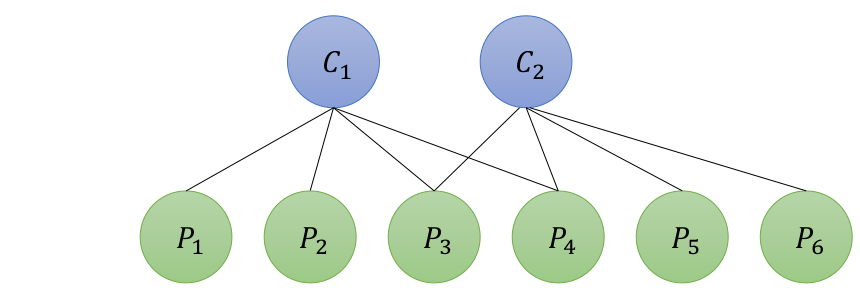
\includegraphics[scale=0.32]{img/node_graph.png}
\end{center}

Then, the overall cost function is  

\begin{align*}
  f(\mathbf{X}) = \frac{1}{2} \Big( ||\mathbf{e}_{11}(\mathbf{X})||^2 + ||\mathbf{e}_{12}(\mathbf{X})||^2 & + ||\mathbf{e}_{13}(\mathbf{X})||^2 + ||\mathbf{e}_{14}(\mathbf{X})||^2 \\ 
  & + ||\mathbf{e}_{23}(\mathbf{X})||^2 + ||\mathbf{e}_{24}(\mathbf{X})||^2 + ||\mathbf{e}_{25}(\mathbf{X})||^2 + ||\mathbf{e}_{26}(\mathbf{X})||^2 \Big)
\end{align*}

Let $\mathbf{J}_{ij}$ be the Jacobian corresponding to $\mathbf{e}_{ij}$, and we can form the Jacobian 
\[\mathbf{J} = \begin{bmatrix} J_{11} \\ J_{12} \\ J_{13} \\ J_{14} \\ J_{23} \\ J_{24} \\ J_{25} \\ J_{26} \end{bmatrix} = \begin{bmatrix} 
\frac{\partial \mathbf{e}_{11}}{\partial \mathbf{x}_1} & \mathbf{0}_{2 \times 6} & \frac{\partial \mathbf{e}_{11}}{\partial \mathbf{y}_1} & \mathbf{0}_{2 \times 3} & \mathbf{0}_{2 \times 3} & \mathbf{0}_{2 \times 3} & \mathbf{0}_{2 \times 3} & \mathbf{0}_{2 \times 3} \\ 
\frac{\partial \mathbf{e}_{12}}{\partial \mathbf{x}_1} & \mathbf{0}_{2 \times 6} & \mathbf{0}_{2 \times 3} & \frac{\partial \mathbf{e}_{12}}{\partial \mathbf{y}_2} & \mathbf{0}_{2 \times 3} & \mathbf{0}_{2 \times 3} & \mathbf{0}_{2 \times 3} & \mathbf{0}_{2 \times 3} \\ 
\frac{\partial \mathbf{e}_{13}}{\partial \mathbf{x}_1} & \mathbf{0}_{2 \times 6} & \mathbf{0}_{2 \times 3} & \mathbf{0}_{2 \times 3} & \frac{\partial \mathbf{e}_{13}}{\partial \mathbf{y}_3} & \mathbf{0}_{2 \times 3} & \mathbf{0}_{2 \times 3} & \mathbf{0}_{2 \times 3} \\ 
\frac{\partial \mathbf{e}_{14}}{\partial \mathbf{x}_1} & \mathbf{0}_{2 \times 6} & \mathbf{0}_{2 \times 3} & \mathbf{0}_{2 \times 3} & \mathbf{0}_{2 \times 3} & \frac{\partial \mathbf{e}_{14}}{\partial \mathbf{y}_4} & \mathbf{0}_{2 \times 3} & \mathbf{0}_{2 \times 3} \\

\mathbf{0}_{2 \times 6} & \frac{\partial \mathbf{e}_{23}}{\partial \mathbf{x}_2}  & \mathbf{0}_{2 \times 3} & \mathbf{0}_{2 \times 3} & \frac{\partial \mathbf{e}_{23}}{\partial \mathbf{y}_3} & \mathbf{0}_{2 \times 3} & \mathbf{0}_{2 \times 3} & \mathbf{0}_{2 \times 3} \\

\mathbf{0}_{2 \times 6} & \frac{\partial \mathbf{e}_{24}}{\partial \mathbf{x}_2}  & \mathbf{0}_{2 \times 3} & \mathbf{0}_{2 \times 3} & \mathbf{0}_{2 \times 3} & \frac{\partial \mathbf{e}_{24}}{\partial \mathbf{y}_3} & \mathbf{0}_{2 \times 3} & \mathbf{0}_{2 \times 3} \\

\mathbf{0}_{2 \times 6} & \frac{\partial \mathbf{e}_{25}}{\partial \mathbf{x}_2} & \mathbf{0}_{2 \times 3} & \mathbf{0}_{2 \times 3} & \mathbf{0}_{2 \times 3} & \mathbf{0}_{2 \times 3} & \frac{\partial \mathbf{e}_{25}}{\partial \mathbf{y}_5} &  \mathbf{0}_{2 \times 3} \\

\mathbf{0}_{2 \times 6} & \frac{\partial \mathbf{e}_{26}}{\partial \mathbf{x}_2}  & \mathbf{0}_{2 \times 3} & \mathbf{0}_{2 \times 3} & \mathbf{0}_{2 \times 3} & \mathbf{0}_{2 \times 3} & \mathbf{0}_{2 \times 3} & \frac{\partial \mathbf{e}_{26}}{\partial \mathbf{y}_6}
\end{bmatrix}\]
and we can compute $\mathbf{H} = \mathbf{J}^T \mathbf{J}$, which will look like an \textit{arrowhead matrix}. Again, with linear algebra techniques, we can invert this and solve the optimization problem. 

\subsection{Robust Kernels}

In this BA problem, we want to minimize the $L_2$ norm of the error term $\mathbf{e}$. This is ideal, but what happens if the data given by a certain error term is wrong due to some mismatch of the nodes? That is, what if we added an edge that shouldn't have been added to the graph? The algorithm will try to incorporate an observation that is impossible to happen, which will contribute to a large error that shouldn't be there. Even worse, the gradient is likely to be very large, too, and this will eliminate out the influence of other correct edges. We can fix this by introducing a robust \textbf{kernel function}, which bounds the error of each edge. More specifically, we can replace the $L_2$ norm with something that is more bounded (whether it'd be the norm itself or its derivatives). For example, we can use the Huber kernel 
\[H(e) = \begin{cases} \frac{1}{2} e^2 & \text{ when } |e| \leq \delta \\ \delta (|e| - \frac{1}{2} \delta) & \text{ otherwise } \end{cases}\]

\subsection{Sliding Window Filter and Optimization}

Solving graph optimization with camera pose and spatial points is called BA, but this often does not meet real time SLAM requirements. This puts a limit on the size of the matrix $\mathbf{H}$, the number of iterations we can compute for the optimization process, and so on. The first way to reduce computation is to extract keyframes from the video, only constructing the BA between the keyframe and the landmarks. The non-keyframes are only used for localization and do not contribute to the mapping point. But as enough time passes, the number of keyframes will also increase to the point where we cannot compute efficiently. 

The simplest way to control the BA is to keep only the $N$ keyframes closest to the current moment and remove the earlier ones. Therefore, we will fix the BA within a time window, and those that leave this window is discarded, hence the name, sliding window filter. This means that the connected graph between the camera poses and the landmarks will be updated. Note that while we will not elaborate here, more sophisticated sliding windows must be implemented rather than just that of closest in time, since a robot stopping in one pose for an extended amount of time may lead to bad degradation errors. 

Remember that given a connected graph of poses $\mathbf{x}_n$ and landmarks $\mathbf{y}_m$, this specific graph corresponds to some sparse block matrix $\mathbf{H}$ that we eventually have to invert. Now, a change to this graph would lead to a change in $\mathbf{H}$, which would affect our optimization scheme. Suppose we have a set of poses $\mathbf{x}_1, \ldots, \mathbf{x}_N$ along with the set of all landmarks that they can see, indexed by some set $J$: $\{\mathbf{y}_j\}_{j \in J}$. Then, a sliding window would refer to an addition of $\mathbf{x}_{N+1}$ and a deletion of $\mathbf{x}_1$, along with the modification of whatever landmarks. 
\begin{enumerate}
    \item It turns out that adding the new pose and keyframe isn't all that difficult, and we can conveniently optimize $\mathbf{H}$ given that new rows/columns are added since we are dealing with bigger Gaussians. 
    \item Deleting a keyframe, along with the landmarks it observes is quite a pain, however. First, it turns out that $\mathbf{H}$ will no longer be sparse, leading to bigger issues. 
\end{enumerate}

\subsection{Pose Graph Optimization}
Given the amount of feature points one can extract from an image, it is unsurprising that landmarks $\mathbf{y}_m$ occupy most of the optimization time. In fact, after several observations, the spatial position of the landmarks will converge to a value and remain almost unchanged (think about 8-point algorithm plus optimization done for countless frames), while the divergent outliers are usually invisible. Optimizing the landmarks seems redundant, so we should focus on pose estimation. That is, we can fix the feature points after a few iterations and regard them as constraints of pose estimation. 

In fact, we can construct a graph optimization with \textit{only} pose variables. The edge between pose vertices can be set with measurements by the ego-motion estimation obtained from feature matching. So once the initial estimation of of the landmark points is completed (by?), we no longer optimize them and only care about the connections between all camera poses. That is, we abandon the optimization of landmark, and only keep the edges between pose variables. This way, we can keep the computational cost low, much better than a simple window filter. When we no longer optimize the landmark in BA and only regard them as constraints on the pose nodes, we get a pose graph with a much reduced scale. 

\begin{center}
    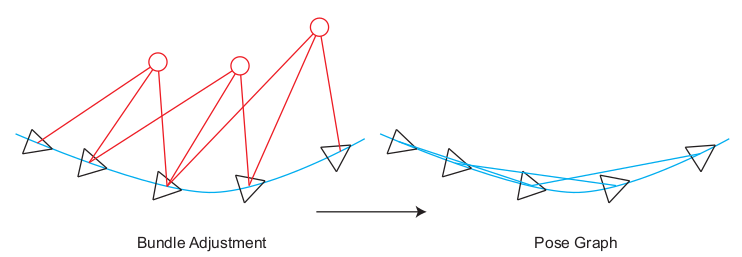
\includegraphics[scale=0.5]{img/pose_optimization.png}
\end{center}

Now let us define the vertices and edges in a pose graph optimization. The node represents the camera pose, denoted $\mathbf{x}_1, \ldots, \mathbf{x}_n$, which we will represent as elements of $\mathrm{SE}(3)$. The edge is the estimation of the relative motion between the two pose nodes, where the movement from $\mathbf{x}_i$ to $\mathbf{x}_j$ is denoted $\Delta \mathbf{x}_{ij} \in \mathrm{SE}(3)$. Note that this movement is really just 
\[\Delta \mathbf{x}_{ij} = \mathbf{x}_{j} \, \mathbf{x}_i^{-1}\]
Since we are working witha fully connected graph of these nodes, these compositions will not be exactly consistent: certain compositions from $\mathbf{x}_i$ to $\mathbf{x}_j$ will not match exactly. So this can just be turned into a least squares problem. Ideally, if both sides of the equation above are equal, we should have 
\[I = (\Delta \mathbf{x}_{ij})^{-1}\mathbf{x}_{j} \, \mathbf{x}_i^{-1}\]
and mapping both sides through the logarithmic map gives us this equation in the Lie algebra $\mathfrak{se}(3)$. 
\[\mathbf{0} = \ln \big(  (\Delta \mathbf{x}_{ij})^{-1}\mathbf{x}_{j} \, \mathbf{x}_i^{-1}\big)\]
Let $\mathbf{e}_{ij} = \ln \big(  (\Delta \mathbf{x}_{ij})^{-1}\mathbf{x}_{j} \, \mathbf{x}_i^{-1}\big)$ be the error of the edge from $\mathbf{x}_i$ to $\mathbf{x}_j$, and our job is to minimize some weighted of these errors $\mathbf{e}_{ij} \in \mathbb{R}^6$. This total error function $C$ of the graph edges $\mathcal{E}$ can be written as 
\[C(\mathcal{E}) \coloneqq \frac{1}{2} \sum_{(i, j) \in \mathcal{E}} \mathbf{e}_{ij}^T \boldsymbol{\Sigma}_{ij}^{-1} \mathbf{e}_{ij}\]
where the $\boldsymbol{\Sigma}_{ij}$'s account for sensitivity in certain edges or components of the error term for each edge. 

\section{SLAM and Beyond}

Let's now summarize what SLAM does. Note that filtering is not used at all in modern SLAM systems, and the following is a very general outline of SLAM. Many variants have modifications. 
\begin{enumerate}
    \item We first take a sequence of images (at a certain framerate) and identify its keyframes. The keyframes are considered the "high-quality" data. 
    \item All frames are used for the frontend, which includes pose estimation and estimation of map points. This is usually done with lightweight algorithms such as the 8 point algorithm or triangulation. The output of this module is some noisy initialization of both the pose estimates $\mathbf{X}$ and the landmark estimates $\mathbf{Y}$. 
    \item The initial estimates are optimized with the backend using more heavy-duty optimization techniques, such as bundle adjustment and (pose) graph optimization. Only the keyframes are needed for this. Indeed, since adjacent frames are similar, deleting them won't lose much information (dimensionality-reduction without much information loss). Furthermore, we can treat this backend as some combination of the backend algorithms mentioned, e.g. graph optimization, filtering, sliding windows, pose graph optimization. However, graph optimization is the most common (at least in ORB-SLAM3). Ultimately, the output of this module is the optimized estimates of $\mathbf{X}$ and $\mathbf{Y}$. 
    \item Then loop closing is done on $\mathbf{X}$ for futher optimization. 
\end{enumerate}

\subsection{Edge SLAM}
All this is computationally quite expensive, so the purpose of EdgeSLAM is to offload the computation and memory overhead to an edge server. Second, we want to keep the overall resource usage (CPU, memory) on the mobile agent to be relatively constant for long-term operation. What it essentially does is keep the tracking module within the mobile agent and outsources the local mapping, loop closing, segmentation, and global map building processes in the edge server. Since tracking requires the mobile agent to compare new frames with previous ones, we keep a local map within the mobile agent. 
\begin{enumerate}
    \item The mobile agent takes in frames and uses feature detection to compare them to its local map. It calculates the relative odometry and selects keyframes to send to the edge server. 
    \item The edge server performs bundle adjustment, loop detection, (possibly segmentation), and builds the global map. Then it sends the relevant portion of the map to the mobile agent, updating its local map. 
\end{enumerate}
This biggest problem now here is bandwidth and latency. More specifically, to achieve SLAM performance at 30fps, we would want the end-to-end latency (mobile to server to mobile) plus the edge processing time to be less than 33.3ms. Here are some solutions for improvement: 
\begin{enumerate}
    \item We utilize three separate connections that work independently of each other so that there is no sequence nor delays (frames sent from agent to server, keyframes sent from agent to server, map updates sent from server to agent). 
    
    \item If traffic is too high, the mobile device can choose to reject the local map update. This reduces the frequency of local map updates (which is time-consuming and pauses the agent from processing new frames), resulting in a slight loss of accuracy. To ensure a minimum frequency of updates, we also implement a time-out mechanism to determine when a local map is stale. 
    
    \item We can tweak parameters that determine the conditions in which we should choose a keyframe. This allows for more or less frequent keyframe updates (what Xu basically does)
    
    \item When updating the map, depending on which is more efficent, we can either 
    \begin{enumerate}
        \item erase the entire local map and update it from scratch, or 
        \item apply edge changes to the local map by "adding" the differences
    \end{enumerate}
\end{enumerate}

\subsection{Multi-Agent Collaborative SLAM}

Now take this a step further, where we utilize edge servers to conduct SLAM with multiple agents. This leads to the potential problems: 
\begin{enumerate}
    \item Increased bandwidth. 
    \item First come first serve queuing can cause significant delay in localization updates. 
    \item The size of the global map increases sharply, which may exceed the memory capabilities of the edge server. 
    \item Overlaps in local maps, so we must develop an efficient way to merge maps. 
\end{enumerate}


\end{document}
